% Additional confirmatory results (Section S6). Reorganized during the journal
% revision (agent S, 2026-10-13) from sections/supplement.tex and
% sections/results.tex of the rule-assembled attempt. Tables and figures of
% the engineering agent (generated/journal-esm-*) replace the rule-assembled
% displays when they exist; the older displays are the fallback.
\def\esmfigboundaries{fig:boundaries-by-model}%
\def\esmfigaucA{fig:auc-A}\def\esmfigaucC{fig:auc-C}\def\esmfigaucD{fig:auc-D}\def\esmfigaucE{fig:auc-E}%

The article reports the boundaries against B (Table~\ref{main-tab:boundaries-B} and Fig.~\ref{main-fig:auc-B}) and summarizes the other persistence models (Table~\ref{main-tab:other-models}). This section gives the full displays behind them, the cell values against B, the secondary targets, the gaps, the controls and sensitivities, and the diagnostics.

\subsection{Boundaries for every persistence model}\label{sec:additional-models}

Table~\ref{tab:v4-T1} gives the first and sustained boundaries for all five persistence models at every $r$, Fig.~\ref{\esmfigboundaries} plots them, and Figs.~\ref{\esmfigaucA}, \ref{\esmfigaucC}, \ref{\esmfigaucD} and~\ref{\esmfigaucE} give the AUC profiles against A, C, D and E (the profiles against B are Fig.~\ref{main-fig:auc-B} of the article).
% Moved from sections/results.tex (Other null families) of the rule-assembled attempt.
All \resultnum{v4.tab.T4.2-all-all-all.units}{36} units of the secondary persistence models finished, and \resultnum{v4.tab.T4.2-all-all-all.valid}{27} were complete and valid. The \resultnum{v4.inv.t2.n_invalid}{9} units of C were complete but invalid: their band at $a=0$ excluded \resultnum{v4.protocol.null_auc}{0.5}, with a zero-strength point AUC of \resultnum{j.models.C.zero_auc.min}{1.000} at every share, and their boundaries are suppressed. The prespecified condition for comparing persistence models required a valid main curve and all 36 secondary units complete and valid; it was not met, so no comparison across models is made, locally or for the whole curve, and no persistence model is promoted or demoted. Valid units remain displayed.
For C, the zero-strength rule is the protocol's operational eligibility rule without a guaranteed identity of the arms at zero strength, because only C's persistence arm receives the altered channel. Its failure reflects that the altered response channel alone separates the panels; by itself it establishes neither an implementation defect nor influence. Read after the results became available: because the two arms of C differ at zero strength by construction, its zero-strength check could pass only if the classifier could not see that difference, and at this panel size it could; the failure is a property of how C was designed, says nothing about persistence and, under the prespecified condition, prevented the comparison across models.
All nine units of D were complete and valid, but every first and sustained boundary against D is censored at a fit gap. The first gap is at $a=\resultnum{j.models.D.r055.first_gap}{0.10}$ at seven shares, at $a=\resultnum{j.models.D.r050.first_gap}{0.01}$ (another solver status) at $r=0.50$ and at $a=\resultnum{j.models.D.r060.first_gap}{0.003}$ (the propagation gap of amendment v4.4) at $r=0.60$. D has \resultnum{j.models.D.gaps.total}{38} gap cells: \resultnum{j.models.D.gaps.family_limit}{33} family limits on the profile, \resultnum{j.models.D.gaps.solver}{4} other solver statuses and \resultnum{j.models.D.gaps.propagation}{1} propagation gap. A family limit on the profile means that the declared profile solver reached the edge of D's parameter box ($\eta\le0.8$; Table~\ref{tab:design-conventions}) without an accepted root for the influence arm's lag-1 and lag-2 correlations. At $a=0.10$ all nine gaps of D are family limits; at $a=0.30$--0.90 the gaps include one other solver status at each of $r=0.55$, 0.70 and 0.80 (\allunitsresource\ gives the gap kinds of every unit). Read after the results became available: within its box, the declared profile solver found no admissible match for D at $a=0.10$ and 0.30 at any share, the strengths where the boundary against B lies. This is a statement about the declared matching procedure. Because the profile is checked for monotonicity only at the points it evaluates (Section~\ref{sec:dd-matching}), it does not establish that no parameter in the box reproduces those moments.
A and E were complete and valid at every share; their boundaries are displayed without a comparison with B.
The prespecified display of offsets between models applies only when the condition for comparing models is met, so it is not reported.

% Generated by ic_study.analysis.v4_report_export from the v4 report with
% manifest SHA-256 6608b3960eb73011caca97870a4ffd3dbfbcd4c2df09bbbcb576c1c9452cf981.
% Edited during the journal revision (agent S, 2026-10-13): captions, headers and
% categorical cells in plain English; every number keeps its \resultnum binding.
\begin{table*}[tp]
\caption{First and sustained boundaries at the primary target AUC 0.70 for every persistence model and signal share (the article shows the B rows in Table~\ref{main-tab:boundaries-B} and the other models in Table~\ref{main-tab:other-models}): status at the close, zero-strength check, number of gap cells, first boundary $a^*$ and sustained boundary $a_s^*$ with their boundary intervals in brackets, and the protocol's region label of $a^*$. Censored at gap $x$: the boundary, and both ends of its interval, cannot be declared across the fit gap at $a=x$ (gap-censoring rule; a sustained boundary censored at 0.9 is not a boundary at 0.9). Suppressed: no boundary because the zero-strength check failed, so the region is none. Regions follow the inherited convention: small, the whole interval within $(0,0.03]$; large, the whole interval above 0.03; indeterminate when $a^*=0$ or the interval crosses 0.03 or has a censored end; censored when the first boundary itself is censored (a label of this resource and Online Resource~2, not used in the article). The 0.03 cut is an inherited convention, not a demonstrated effect size. Grid values are printed as released (0.1 means 0.10). Models: A autoregressive; B trait plus autoregressive; C autoregressive with an altered response channel; D state-dependent; E mover--stayer. Status: CV complete and valid; CI complete but invalid. $a=0$ check: the zero-strength check. \dag\ $r=0.70$, examined during calibration. Secondary targets: Table~\ref{tab:v4-sec}; gap kinds: Tables~\ref{tab:v4-sgaps} and~\ref{tab:v4-T4}.}\label{tab:v4-T1}
\centering\scriptsize
\setlength{\tabcolsep}{2pt}
\begin{tabular}{lrllrp{2.9cm}p{2.9cm}l}
\toprule
Model & $r$ & Status & $a=0$ check & Gaps & $a^*$ [interval] & $a_s^*$ [interval] & Region \\
\midrule
B & \resultnum{v4.tab.T1.B.r050.r}{0.50} & CV & passed & \resultnum{v4.tab.T1.B.r050.gaps}{0} & \resultnum{v4.tab.T1.B.r050.a_star.1}{0.3} [\resultnum{v4.tab.T1.B.r050.a_star.2}{0.1}, \resultnum{v4.tab.T1.B.r050.a_star.3}{0.3}] & \resultnum{v4.tab.T1.B.r050.a_s_star.1}{0.3} [\resultnum{v4.tab.T1.B.r050.a_s_star.2}{0.1}, \resultnum{v4.tab.T1.B.r050.a_s_star.3}{0.3}] & large \\
B & \resultnum{v4.tab.T1.B.r055.r}{0.55} & CV & passed & \resultnum{v4.tab.T1.B.r055.gaps}{2} & \resultnum{v4.tab.T1.B.r055.a_star.1}{0.1} [\resultnum{v4.tab.T1.B.r055.a_star.2}{0.1}, \resultnum{v4.tab.T1.B.r055.a_star.3}{0.3}] & censored at gap \resultnum{v4.tab.T1.B.r055.a_s_star.1}{0.9} & large \\
B & \resultnum{v4.tab.T1.B.r060.r}{0.60} & CV & passed & \resultnum{v4.tab.T1.B.r060.gaps}{0} & \resultnum{v4.tab.T1.B.r060.a_star.1}{0.1} [\resultnum{v4.tab.T1.B.r060.a_star.2}{0.1}, \resultnum{v4.tab.T1.B.r060.a_star.3}{0.3}] & \resultnum{v4.tab.T1.B.r060.a_s_star.1}{0.1} [\resultnum{v4.tab.T1.B.r060.a_s_star.2}{0.1}, \resultnum{v4.tab.T1.B.r060.a_s_star.3}{0.3}] & large \\
B & \resultnum{v4.tab.T1.B.r065.r}{0.65} & CV & passed & \resultnum{v4.tab.T1.B.r065.gaps}{0} & \resultnum{v4.tab.T1.B.r065.a_star.1}{0.1} [\resultnum{v4.tab.T1.B.r065.a_star.2}{0.1}, \resultnum{v4.tab.T1.B.r065.a_star.3}{0.1}] & \resultnum{v4.tab.T1.B.r065.a_s_star.1}{0.1} [\resultnum{v4.tab.T1.B.r065.a_s_star.2}{0.1}, \resultnum{v4.tab.T1.B.r065.a_s_star.3}{0.1}] & large \\
B & \resultnum{v4.tab.T1.B.r070.r}{0.70}\dag{} & CV & passed & \resultnum{v4.tab.T1.B.r070.gaps}{1} & \resultnum{v4.tab.T1.B.r070.a_star.1}{0.1} [\resultnum{v4.tab.T1.B.r070.a_star.2}{0.1}, \resultnum{v4.tab.T1.B.r070.a_star.3}{0.1}] & censored at gap \resultnum{v4.tab.T1.B.r070.a_s_star.1}{0.9} & large \\
B & \resultnum{v4.tab.T1.B.r075.r}{0.75} & CV & passed & \resultnum{v4.tab.T1.B.r075.gaps}{0} & \resultnum{v4.tab.T1.B.r075.a_star.1}{0.1} [\resultnum{v4.tab.T1.B.r075.a_star.2}{0.1}, \resultnum{v4.tab.T1.B.r075.a_star.3}{0.1}] & \resultnum{v4.tab.T1.B.r075.a_s_star.1}{0.1} [\resultnum{v4.tab.T1.B.r075.a_s_star.2}{0.1}, \resultnum{v4.tab.T1.B.r075.a_s_star.3}{0.1}] & large \\
B & \resultnum{v4.tab.T1.B.r080.r}{0.80} & CV & passed & \resultnum{v4.tab.T1.B.r080.gaps}{0} & \resultnum{v4.tab.T1.B.r080.a_star.1}{0.1} [\resultnum{v4.tab.T1.B.r080.a_star.2}{0.1}, \resultnum{v4.tab.T1.B.r080.a_star.3}{0.1}] & \resultnum{v4.tab.T1.B.r080.a_s_star.1}{0.1} [\resultnum{v4.tab.T1.B.r080.a_s_star.2}{0.1}, \resultnum{v4.tab.T1.B.r080.a_s_star.3}{0.1}] & large \\
B & \resultnum{v4.tab.T1.B.r085.r}{0.85} & CV & passed & \resultnum{v4.tab.T1.B.r085.gaps}{0} & \resultnum{v4.tab.T1.B.r085.a_star.1}{0.1} [\resultnum{v4.tab.T1.B.r085.a_star.2}{0.1}, \resultnum{v4.tab.T1.B.r085.a_star.3}{0.1}] & \resultnum{v4.tab.T1.B.r085.a_s_star.1}{0.1} [\resultnum{v4.tab.T1.B.r085.a_s_star.2}{0.1}, \resultnum{v4.tab.T1.B.r085.a_s_star.3}{0.1}] & large \\
B & \resultnum{v4.tab.T1.B.r090.r}{0.90} & CV & passed & \resultnum{v4.tab.T1.B.r090.gaps}{0} & \resultnum{v4.tab.T1.B.r090.a_star.1}{0.1} [\resultnum{v4.tab.T1.B.r090.a_star.2}{0.1}, \resultnum{v4.tab.T1.B.r090.a_star.3}{0.1}] & \resultnum{v4.tab.T1.B.r090.a_s_star.1}{0.1} [\resultnum{v4.tab.T1.B.r090.a_s_star.2}{0.1}, \resultnum{v4.tab.T1.B.r090.a_s_star.3}{0.1}] & large \\
A & \resultnum{v4.tab.T1.A.r050.r}{0.50} & CV & passed & \resultnum{v4.tab.T1.A.r050.gaps}{0} & \resultnum{v4.tab.T1.A.r050.a_star.1}{0.3} [\resultnum{v4.tab.T1.A.r050.a_star.2}{0.1}, \resultnum{v4.tab.T1.A.r050.a_star.3}{0.3}] & \resultnum{v4.tab.T1.A.r050.a_s_star.1}{0.3} [\resultnum{v4.tab.T1.A.r050.a_s_star.2}{0.1}, \resultnum{v4.tab.T1.A.r050.a_s_star.3}{0.3}] & large \\
A & \resultnum{v4.tab.T1.A.r055.r}{0.55} & CV & passed & \resultnum{v4.tab.T1.A.r055.gaps}{0} & \resultnum{v4.tab.T1.A.r055.a_star.1}{0.1} [\resultnum{v4.tab.T1.A.r055.a_star.2}{0.1}, \resultnum{v4.tab.T1.A.r055.a_star.3}{0.3}] & \resultnum{v4.tab.T1.A.r055.a_s_star.1}{0.1} [\resultnum{v4.tab.T1.A.r055.a_s_star.2}{0.1}, \resultnum{v4.tab.T1.A.r055.a_s_star.3}{0.3}] & large \\
A & \resultnum{v4.tab.T1.A.r060.r}{0.60} & CV & passed & \resultnum{v4.tab.T1.A.r060.gaps}{0} & \resultnum{v4.tab.T1.A.r060.a_star.1}{0.1} [\resultnum{v4.tab.T1.A.r060.a_star.2}{0.1}, \resultnum{v4.tab.T1.A.r060.a_star.3}{0.1}] & \resultnum{v4.tab.T1.A.r060.a_s_star.1}{0.1} [\resultnum{v4.tab.T1.A.r060.a_s_star.2}{0.1}, \resultnum{v4.tab.T1.A.r060.a_s_star.3}{0.1}] & large \\
A & \resultnum{v4.tab.T1.A.r065.r}{0.65} & CV & passed & \resultnum{v4.tab.T1.A.r065.gaps}{0} & \resultnum{v4.tab.T1.A.r065.a_star.1}{0.1} [\resultnum{v4.tab.T1.A.r065.a_star.2}{0.1}, \resultnum{v4.tab.T1.A.r065.a_star.3}{0.1}] & \resultnum{v4.tab.T1.A.r065.a_s_star.1}{0.1} [\resultnum{v4.tab.T1.A.r065.a_s_star.2}{0.1}, \resultnum{v4.tab.T1.A.r065.a_s_star.3}{0.1}] & large \\
A & \resultnum{v4.tab.T1.A.r070.r}{0.70}\dag{} & CV & passed & \resultnum{v4.tab.T1.A.r070.gaps}{0} & \resultnum{v4.tab.T1.A.r070.a_star.1}{0.1} [\resultnum{v4.tab.T1.A.r070.a_star.2}{0.1}, \resultnum{v4.tab.T1.A.r070.a_star.3}{0.1}] & \resultnum{v4.tab.T1.A.r070.a_s_star.1}{0.1} [\resultnum{v4.tab.T1.A.r070.a_s_star.2}{0.1}, \resultnum{v4.tab.T1.A.r070.a_s_star.3}{0.1}] & large \\
A & \resultnum{v4.tab.T1.A.r075.r}{0.75} & CV & passed & \resultnum{v4.tab.T1.A.r075.gaps}{0} & \resultnum{v4.tab.T1.A.r075.a_star.1}{0.1} [\resultnum{v4.tab.T1.A.r075.a_star.2}{0.1}, \resultnum{v4.tab.T1.A.r075.a_star.3}{0.1}] & \resultnum{v4.tab.T1.A.r075.a_s_star.1}{0.1} [\resultnum{v4.tab.T1.A.r075.a_s_star.2}{0.1}, \resultnum{v4.tab.T1.A.r075.a_s_star.3}{0.1}] & large \\
A & \resultnum{v4.tab.T1.A.r080.r}{0.80} & CV & passed & \resultnum{v4.tab.T1.A.r080.gaps}{0} & \resultnum{v4.tab.T1.A.r080.a_star.1}{0.1} [\resultnum{v4.tab.T1.A.r080.a_star.2}{0.1}, \resultnum{v4.tab.T1.A.r080.a_star.3}{0.1}] & \resultnum{v4.tab.T1.A.r080.a_s_star.1}{0.1} [\resultnum{v4.tab.T1.A.r080.a_s_star.2}{0.1}, \resultnum{v4.tab.T1.A.r080.a_s_star.3}{0.1}] & large \\
A & \resultnum{v4.tab.T1.A.r085.r}{0.85} & CV & passed & \resultnum{v4.tab.T1.A.r085.gaps}{0} & \resultnum{v4.tab.T1.A.r085.a_star.1}{0.1} [\resultnum{v4.tab.T1.A.r085.a_star.2}{0.1}, \resultnum{v4.tab.T1.A.r085.a_star.3}{0.1}] & \resultnum{v4.tab.T1.A.r085.a_s_star.1}{0.1} [\resultnum{v4.tab.T1.A.r085.a_s_star.2}{0.1}, \resultnum{v4.tab.T1.A.r085.a_s_star.3}{0.1}] & large \\
A & \resultnum{v4.tab.T1.A.r090.r}{0.90} & CV & passed & \resultnum{v4.tab.T1.A.r090.gaps}{0} & \resultnum{v4.tab.T1.A.r090.a_star.1}{0.1} [\resultnum{v4.tab.T1.A.r090.a_star.2}{0.1}, \resultnum{v4.tab.T1.A.r090.a_star.3}{0.1}] & \resultnum{v4.tab.T1.A.r090.a_s_star.1}{0.1} [\resultnum{v4.tab.T1.A.r090.a_s_star.2}{0.1}, \resultnum{v4.tab.T1.A.r090.a_s_star.3}{0.1}] & large \\
C & \resultnum{v4.tab.T1.C.r050.r}{0.50} & CI & failed & \resultnum{v4.tab.T1.C.r050.gaps}{1} & suppressed & suppressed & none \\
C & \resultnum{v4.tab.T1.C.r055.r}{0.55} & CI & failed & \resultnum{v4.tab.T1.C.r055.gaps}{2} & suppressed & suppressed & none \\
C & \resultnum{v4.tab.T1.C.r060.r}{0.60} & CI & failed & \resultnum{v4.tab.T1.C.r060.gaps}{2} & suppressed & suppressed & none \\
C & \resultnum{v4.tab.T1.C.r065.r}{0.65} & CI & failed & \resultnum{v4.tab.T1.C.r065.gaps}{2} & suppressed & suppressed & none \\
C & \resultnum{v4.tab.T1.C.r070.r}{0.70}\dag{} & CI & failed & \resultnum{v4.tab.T1.C.r070.gaps}{3} & suppressed & suppressed & none \\
C & \resultnum{v4.tab.T1.C.r075.r}{0.75} & CI & failed & \resultnum{v4.tab.T1.C.r075.gaps}{3} & suppressed & suppressed & none \\
C & \resultnum{v4.tab.T1.C.r080.r}{0.80} & CI & failed & \resultnum{v4.tab.T1.C.r080.gaps}{3} & suppressed & suppressed & none \\
C & \resultnum{v4.tab.T1.C.r085.r}{0.85} & CI & failed & \resultnum{v4.tab.T1.C.r085.gaps}{3} & suppressed & suppressed & none \\
C & \resultnum{v4.tab.T1.C.r090.r}{0.90} & CI & failed & \resultnum{v4.tab.T1.C.r090.gaps}{3} & suppressed & suppressed & none \\
\botrule
\end{tabular}
\end{table*}
\begin{table*}[tp]
\addtocounter{table}{-\csname @ne\endcsname}
\providecommand{\theHtable}{\thetable}
\renewcommand{\theHtable}{v4-T1-part1}
\caption{First and sustained boundaries for every persistence model (continued)}\label{tab:v4-T1-part1}
\centering\scriptsize
\setlength{\tabcolsep}{2pt}
\begin{tabular}{lrllrp{2.9cm}p{2.9cm}l}
\toprule
Model & $r$ & Status & $a=0$ check & Gaps & $a^*$ [interval] & $a_s^*$ [interval] & Region \\
\midrule
D & \resultnum{v4.tab.T1.D.r050.r}{0.50} & CV & passed & \resultnum{v4.tab.T1.D.r050.gaps}{5} & censored at gap \resultnum{v4.tab.T1.D.r050.a_star.1}{0.01} & censored at gap \resultnum{v4.tab.T1.D.r050.a_s_star.1}{0.9} & censored \\
D & \resultnum{v4.tab.T1.D.r055.r}{0.55} & CV & passed & \resultnum{v4.tab.T1.D.r055.gaps}{4} & censored at gap \resultnum{v4.tab.T1.D.r055.a_star.1}{0.1} & censored at gap \resultnum{v4.tab.T1.D.r055.a_s_star.1}{0.9} & censored \\
D & \resultnum{v4.tab.T1.D.r060.r}{0.60} & CV & passed & \resultnum{v4.tab.T1.D.r060.gaps}{5} & censored at gap \resultnum{v4.tab.T1.D.r060.a_star.1}{0.003} & censored at gap \resultnum{v4.tab.T1.D.r060.a_s_star.1}{0.9} & censored \\
D & \resultnum{v4.tab.T1.D.r065.r}{0.65} & CV & passed & \resultnum{v4.tab.T1.D.r065.gaps}{4} & censored at gap \resultnum{v4.tab.T1.D.r065.a_star.1}{0.1} & censored at gap \resultnum{v4.tab.T1.D.r065.a_s_star.1}{0.9} & censored \\
D & \resultnum{v4.tab.T1.D.r070.r}{0.70}\dag{} & CV & passed & \resultnum{v4.tab.T1.D.r070.gaps}{4} & censored at gap \resultnum{v4.tab.T1.D.r070.a_star.1}{0.1} & censored at gap \resultnum{v4.tab.T1.D.r070.a_s_star.1}{0.9} & censored \\
D & \resultnum{v4.tab.T1.D.r075.r}{0.75} & CV & passed & \resultnum{v4.tab.T1.D.r075.gaps}{4} & censored at gap \resultnum{v4.tab.T1.D.r075.a_star.1}{0.1} & censored at gap \resultnum{v4.tab.T1.D.r075.a_s_star.1}{0.9} & censored \\
D & \resultnum{v4.tab.T1.D.r080.r}{0.80} & CV & passed & \resultnum{v4.tab.T1.D.r080.gaps}{4} & censored at gap \resultnum{v4.tab.T1.D.r080.a_star.1}{0.1} & censored at gap \resultnum{v4.tab.T1.D.r080.a_s_star.1}{0.9} & censored \\
D & \resultnum{v4.tab.T1.D.r085.r}{0.85} & CV & passed & \resultnum{v4.tab.T1.D.r085.gaps}{4} & censored at gap \resultnum{v4.tab.T1.D.r085.a_star.1}{0.1} & censored at gap \resultnum{v4.tab.T1.D.r085.a_s_star.1}{0.9} & censored \\
D & \resultnum{v4.tab.T1.D.r090.r}{0.90} & CV & passed & \resultnum{v4.tab.T1.D.r090.gaps}{4} & censored at gap \resultnum{v4.tab.T1.D.r090.a_star.1}{0.1} & censored at gap \resultnum{v4.tab.T1.D.r090.a_s_star.1}{0.9} & censored \\
E & \resultnum{v4.tab.T1.E.r050.r}{0.50} & CV & passed & \resultnum{v4.tab.T1.E.r050.gaps}{0} & \resultnum{v4.tab.T1.E.r050.a_star.1}{0.3} [\resultnum{v4.tab.T1.E.r050.a_star.2}{0.1}, \resultnum{v4.tab.T1.E.r050.a_star.3}{0.3}] & \resultnum{v4.tab.T1.E.r050.a_s_star.1}{0.3} [\resultnum{v4.tab.T1.E.r050.a_s_star.2}{0.1}, \resultnum{v4.tab.T1.E.r050.a_s_star.3}{0.3}] & large \\
E & \resultnum{v4.tab.T1.E.r055.r}{0.55} & CV & passed & \resultnum{v4.tab.T1.E.r055.gaps}{2} & \resultnum{v4.tab.T1.E.r055.a_star.1}{0.3} [\resultnum{v4.tab.T1.E.r055.a_star.2}{0.1}, \resultnum{v4.tab.T1.E.r055.a_star.3}{0.3}] & censored at gap \resultnum{v4.tab.T1.E.r055.a_s_star.1}{0.9} & large \\
E & \resultnum{v4.tab.T1.E.r060.r}{0.60} & CV & passed & \resultnum{v4.tab.T1.E.r060.gaps}{0} & \resultnum{v4.tab.T1.E.r060.a_star.1}{0.3} [\resultnum{v4.tab.T1.E.r060.a_star.2}{0.1}, \resultnum{v4.tab.T1.E.r060.a_star.3}{0.3}] & \resultnum{v4.tab.T1.E.r060.a_s_star.1}{0.3} [\resultnum{v4.tab.T1.E.r060.a_s_star.2}{0.1}, \resultnum{v4.tab.T1.E.r060.a_s_star.3}{0.3}] & large \\
E & \resultnum{v4.tab.T1.E.r065.r}{0.65} & CV & passed & \resultnum{v4.tab.T1.E.r065.gaps}{0} & \resultnum{v4.tab.T1.E.r065.a_star.1}{0.1} [\resultnum{v4.tab.T1.E.r065.a_star.2}{0.1}, \resultnum{v4.tab.T1.E.r065.a_star.3}{0.3}] & \resultnum{v4.tab.T1.E.r065.a_s_star.1}{0.1} [\resultnum{v4.tab.T1.E.r065.a_s_star.2}{0.1}, \resultnum{v4.tab.T1.E.r065.a_s_star.3}{0.3}] & large \\
E & \resultnum{v4.tab.T1.E.r070.r}{0.70}\dag{} & CV & passed & \resultnum{v4.tab.T1.E.r070.gaps}{1} & \resultnum{v4.tab.T1.E.r070.a_star.1}{0.1} [\resultnum{v4.tab.T1.E.r070.a_star.2}{0.1}, \resultnum{v4.tab.T1.E.r070.a_star.3}{0.3}] & censored at gap \resultnum{v4.tab.T1.E.r070.a_s_star.1}{0.9} & large \\
E & \resultnum{v4.tab.T1.E.r075.r}{0.75} & CV & passed & \resultnum{v4.tab.T1.E.r075.gaps}{0} & \resultnum{v4.tab.T1.E.r075.a_star.1}{0.1} [\resultnum{v4.tab.T1.E.r075.a_star.2}{0.1}, \resultnum{v4.tab.T1.E.r075.a_star.3}{0.3}] & \resultnum{v4.tab.T1.E.r075.a_s_star.1}{0.1} [\resultnum{v4.tab.T1.E.r075.a_s_star.2}{0.1}, \resultnum{v4.tab.T1.E.r075.a_s_star.3}{0.3}] & large \\
E & \resultnum{v4.tab.T1.E.r080.r}{0.80} & CV & passed & \resultnum{v4.tab.T1.E.r080.gaps}{0} & \resultnum{v4.tab.T1.E.r080.a_star.1}{0.1} [\resultnum{v4.tab.T1.E.r080.a_star.2}{0.1}, \resultnum{v4.tab.T1.E.r080.a_star.3}{0.1}] & \resultnum{v4.tab.T1.E.r080.a_s_star.1}{0.1} [\resultnum{v4.tab.T1.E.r080.a_s_star.2}{0.1}, \resultnum{v4.tab.T1.E.r080.a_s_star.3}{0.1}] & large \\
E & \resultnum{v4.tab.T1.E.r085.r}{0.85} & CV & passed & \resultnum{v4.tab.T1.E.r085.gaps}{0} & \resultnum{v4.tab.T1.E.r085.a_star.1}{0.1} [\resultnum{v4.tab.T1.E.r085.a_star.2}{0.1}, \resultnum{v4.tab.T1.E.r085.a_star.3}{0.1}] & \resultnum{v4.tab.T1.E.r085.a_s_star.1}{0.1} [\resultnum{v4.tab.T1.E.r085.a_s_star.2}{0.1}, \resultnum{v4.tab.T1.E.r085.a_s_star.3}{0.1}] & large \\
E & \resultnum{v4.tab.T1.E.r090.r}{0.90} & CV & passed & \resultnum{v4.tab.T1.E.r090.gaps}{0} & \resultnum{v4.tab.T1.E.r090.a_star.1}{0.1} [\resultnum{v4.tab.T1.E.r090.a_star.2}{0.1}, \resultnum{v4.tab.T1.E.r090.a_star.3}{0.1}] & \resultnum{v4.tab.T1.E.r090.a_s_star.1}{0.1} [\resultnum{v4.tab.T1.E.r090.a_s_star.2}{0.1}, \resultnum{v4.tab.T1.E.r090.a_s_star.3}{0.1}] & large \\
\botrule
\end{tabular}
\end{table*}

\begin{figure}[tp]
\centering
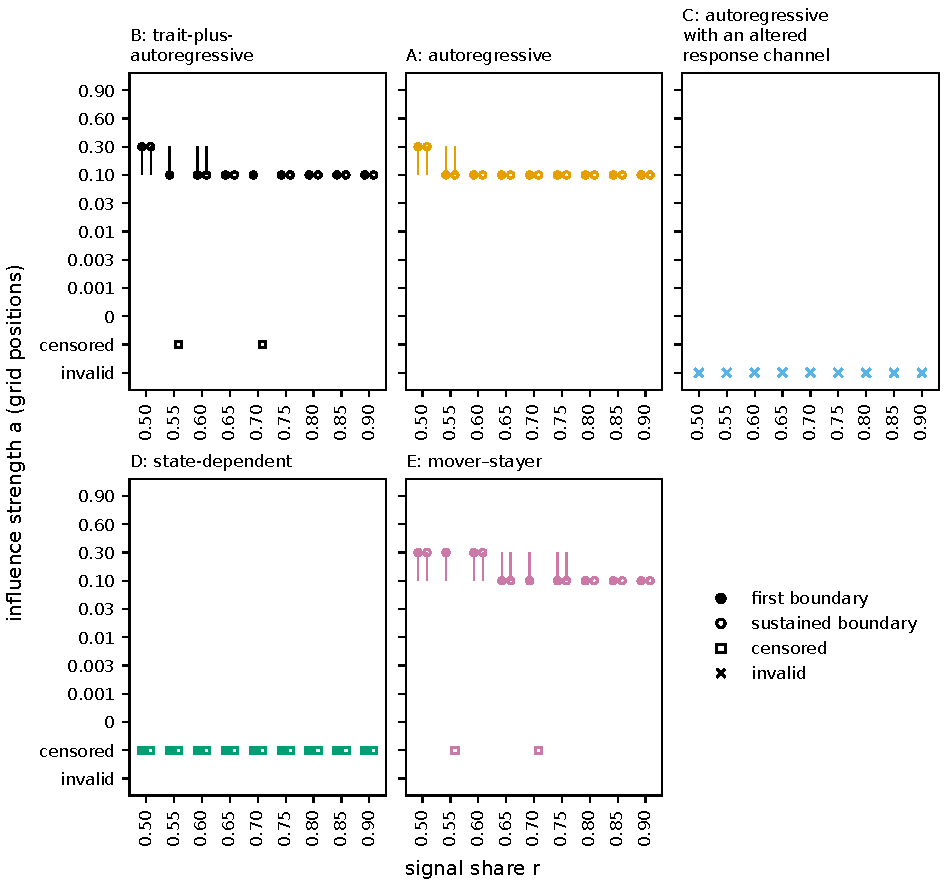
\includegraphics[width=\textwidth]{generated/J1_boundaries_by_model.pdf}
\caption{First and sustained boundaries by persistence model and signal share. Censored boundaries and invalid units occupy separate rows. Filled and open markers distinguish first and sustained boundaries.}\label{fig:boundaries-by-model}
\end{figure}

\begin{figure}[tp]
\centering
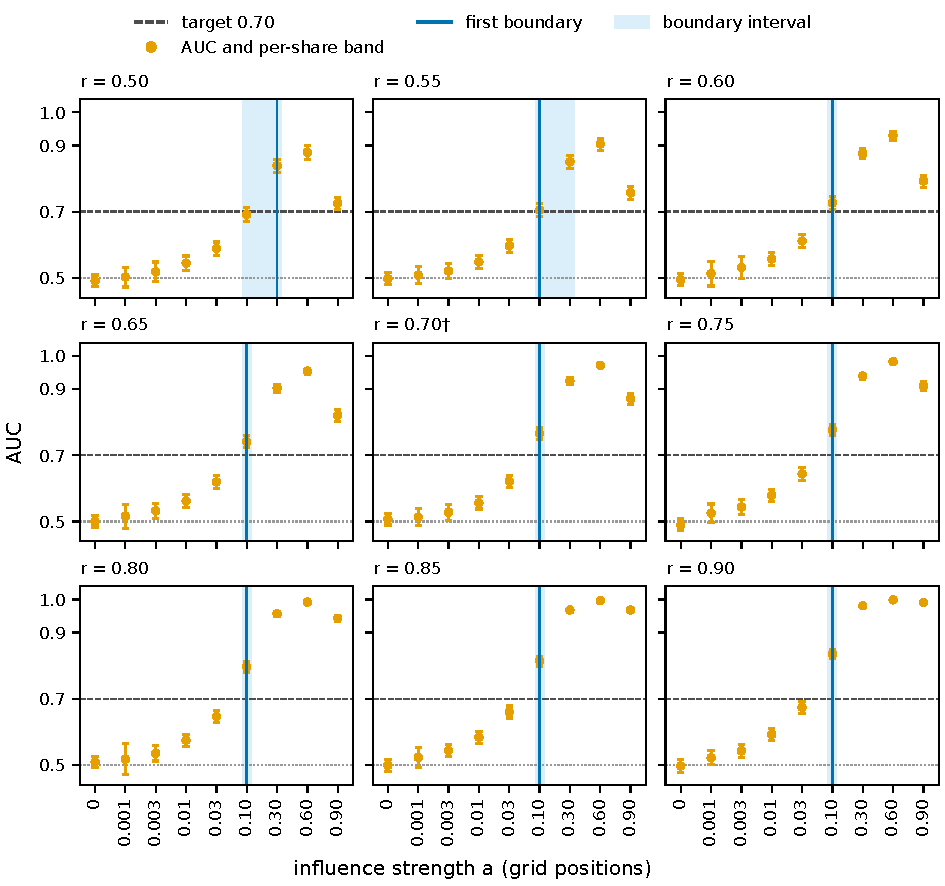
\includegraphics[width=\textwidth]{generated/J2_auc_profiles_A.pdf}
\caption{AUC profiles against autoregressive persistence (A). Vertical bars show per-share bands and crosses mark fit gaps. The target is \resultnum{j.target.r070}{0.70}. $\dag$ Examined during calibration.}\label{fig:auc-A}
\end{figure}
\begin{figure}[tp]
\centering
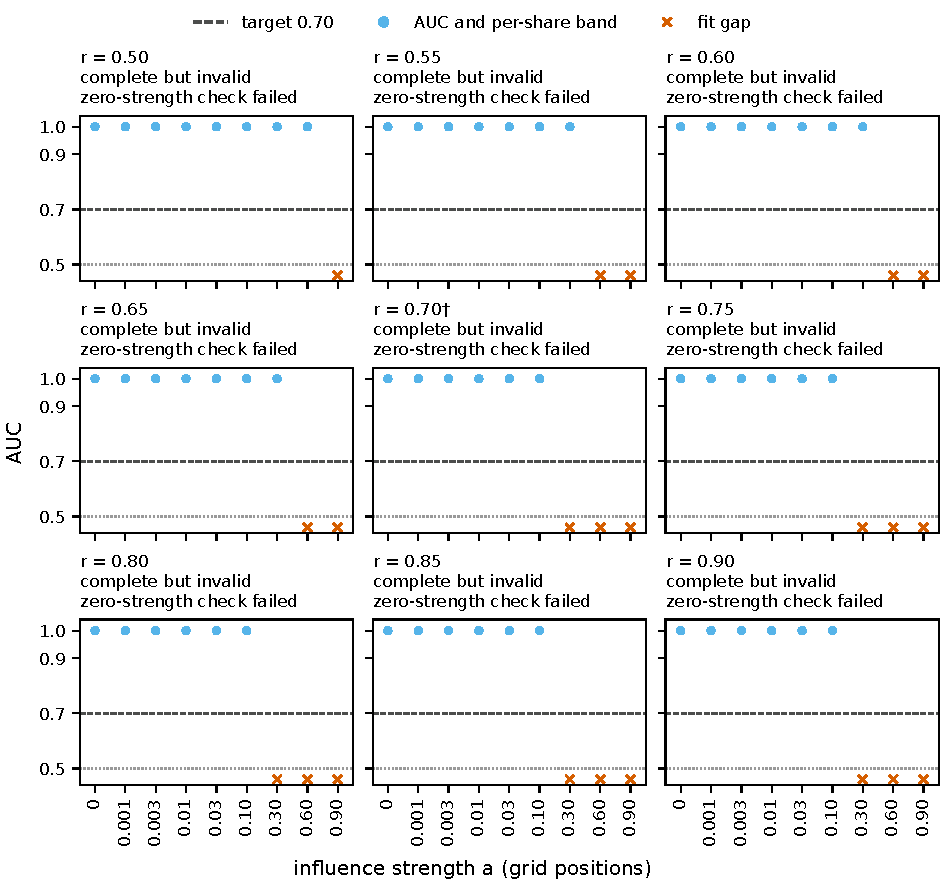
\includegraphics[width=\textwidth]{generated/J2_auc_profiles_C.pdf}
\caption{AUC profiles against autoregressive persistence with an altered response channel (C). Vertical bars show per-share bands and crosses mark fit gaps. The target is \resultnum{j.target.r070}{0.70}. $\dag$ Examined during calibration.}\label{fig:auc-C}
\end{figure}
\begin{figure}[tp]
\centering
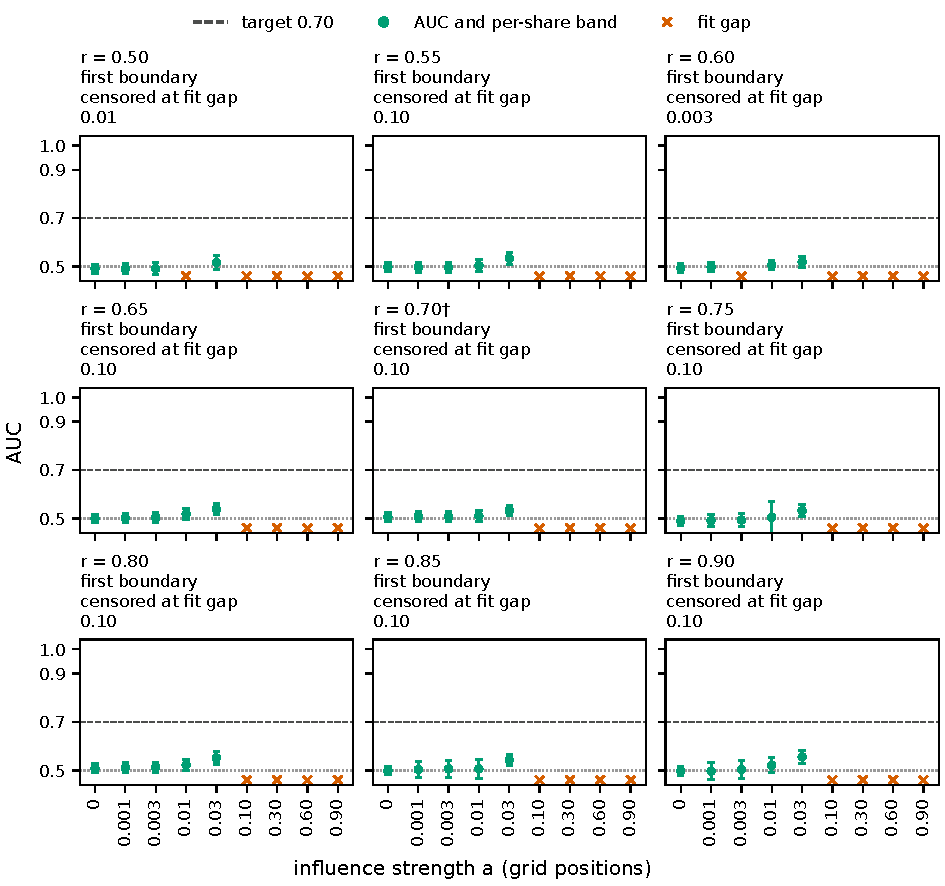
\includegraphics[width=\textwidth]{generated/J2_auc_profiles_D.pdf}
\caption{AUC profiles against state-dependent persistence (D). Vertical bars show per-share bands and crosses mark fit gaps. The target is \resultnum{j.target.r070}{0.70}. $\dag$ Examined during calibration.}\label{fig:auc-D}
\end{figure}
\begin{figure}[tp]
\centering
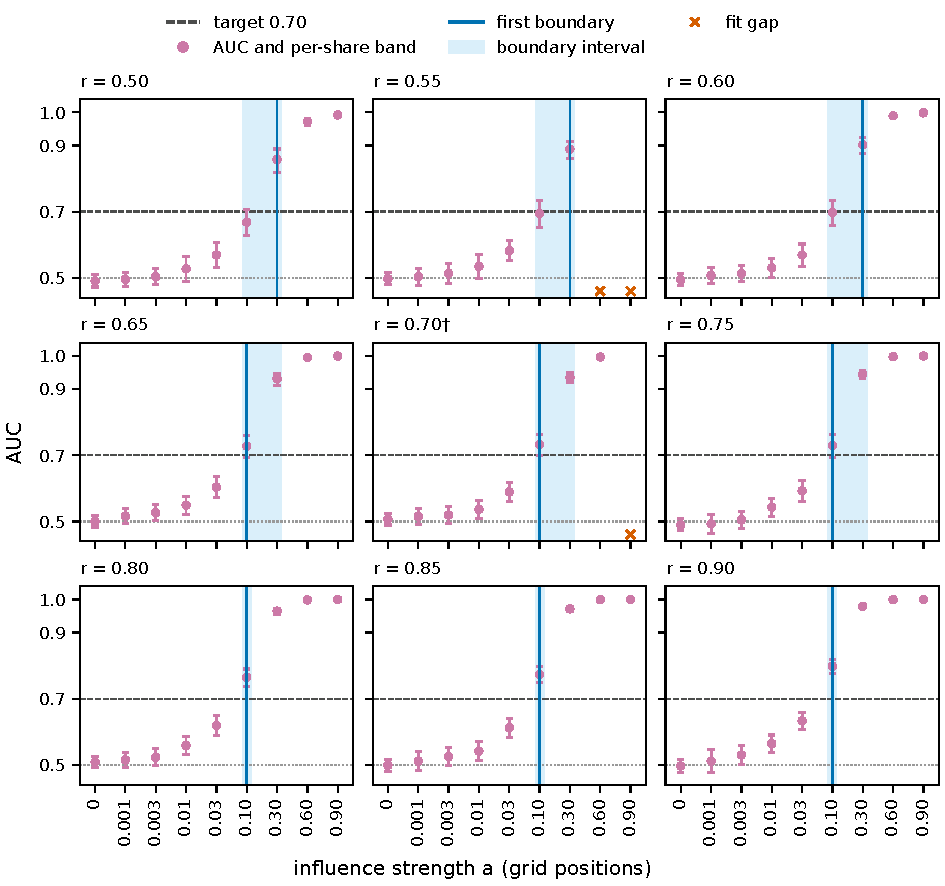
\includegraphics[width=\textwidth]{generated/J2_auc_profiles_E.pdf}
\caption{AUC profiles against mover--stayer persistence (E). Vertical bars show per-share bands and crosses mark fit gaps. The target is \resultnum{j.target.r070}{0.70}. $\dag$ Examined during calibration.}\label{fig:auc-E}
\end{figure}


% Generated by ic_study.analysis.v4_report_export from the v4 report with
% manifest SHA-256 6608b3960eb73011caca97870a4ffd3dbfbcd4c2df09bbbcb576c1c9452cf981. Export again instead of editing this file.
% MECHANISMS permission is absent, so P7 and F3 do not apply.


\subsection{Cells against B, secondary targets and low strengths}\label{sec:additional-b}

Tables~\ref{tab:b-cells}--\ref{tab:b-cells-part-c} list, for each of the 81 cells against B, the point AUC and the limits of the per-share simultaneous band, with the critical value of each share.
The score and nuisance standard errors of each cell, the fitted parameters, fit statuses and retries of the persistence model in each cell, and the mean lag correlations of each cell are absent from the released artifacts used for this resource (the public projection of the released curves and the values catalog), so they are not tabulated here; the band limits carry the combined uncertainty. Unlike these artifacts, the archived released curves hold each cell's fitted parameters, nuisance variance and fit attempts, with their statuses and retries, but not the score standard errors or mean lag correlations; the per-panel features stay in the sealed store (Section~\ref{sec:odd}, Observation). Read after the results became available: the point AUC at $a=\resultnum{j.grid.a1000}{0.10}$ rose from \resultnum{j.b.a1000.auc.min}{0.668} at $r=\resultnum{j.b.a1000.auc.min.r}{0.50}$ to \resultnum{j.b.a1000.auc.max}{0.831} at $r=\resultnum{j.b.a1000.auc.max.r}{0.90}$, and the upper band at $a=\resultnum{j.grid.a0300}{0.03}$ came closest to 0.70 at $r=\resultnum{j.b.a0300.upper.max.r}{0.90}$, where it reached \resultnum{j.b.a0300.upper.max}{0.675}, \resultnum{j.b.a0300.upper.distance_to_target}{0.025} below the target. At $a=0.03$ every lower band already lay above 0.5, while every upper band lay below 0.70 (Tables~\ref{tab:b-cells}--\ref{tab:b-cells-part-c}): the first boundary marks where the expected AUC reaches the 0.70 target, not the first strength at which the band excludes 0.5.

% Moved from sections/supplement.tex (Secondary-target boundaries) of the rule-assembled attempt.
Boundaries for the secondary targets were derived from the released bands using the same inclusive inversion and gap censoring. They were attained at \resultnum{v4.t1.sec060.n_attained}{9} values of $r$ for AUC \resultnum{v4.protocol.secondary_target.lower}{0.60} and at \resultnum{v4.t1.sec080.n_attained}{9} for AUC \resultnum{v4.protocol.secondary_target.upper}{0.80} (Table~\ref{tab:v4-sec}). At AUC 0.60 the first boundary against B was $a=\resultnum{j.b.r075.target060.point}{0.03}$ at $r=0.75$--0.90, with the interval reaching $a=\resultnum{v4.tab.T1sec.B.r090.a060.2}{0.01}$ at $r=0.90$, and $a=\resultnum{j.b.r050.target060.point}{0.10}$ at the lower shares; at AUC 0.80 it was $a=\resultnum{j.b.r050.target080.point}{0.30}$ at $r=0.50$--0.85 and $a=\resultnum{j.b.r090.target080.point}{0.10}$ at $r=0.90$. These targets are secondary and do not replace the primary target; they show that the region label of a boundary depends on the target.
The prespecified table of low-strength cells applies only when a first boundary against B lies at one of the first two positive strengths, $a=0.001$ or 0.003; none does, so it is not reported.

\begin{table}[tp]
\caption{AUC estimates and per-share bands against trait-plus-autoregressive persistence.}\label{tab:b-cells}
\centering\scriptsize
\setlength{\tabcolsep}{2pt}
\begin{tabular}{rrrrrr>{\raggedright\arraybackslash}p{34mm}}
\toprule
$r$ & $a$ & AUC & \shortstack{Lower\\band} & \shortstack{Upper\\band} & Critical & Cell state \\
\midrule
\resultnum{v4.tab.T1.B.r050.r}{0.50} & \resultnum{j.grid.a0000}{0} & \resultnum{j.b.r050.a0000.auc}{0.491} & \resultnum{j.b.r050.a0000.lower}{0.472} & \resultnum{j.b.r050.a0000.upper}{0.509} & \resultnum{j.b.r050.critical}{2.799} & available \\
\resultnum{v4.tab.T1.B.r050.r}{0.50} & \resultnum{j.grid.a0010}{0.001} & \resultnum{j.b.r050.a0010.auc}{0.498} & \resultnum{j.b.r050.a0010.lower}{0.474} & \resultnum{j.b.r050.a0010.upper}{0.523} & \resultnum{j.b.r050.critical}{2.799} & available \\
\resultnum{v4.tab.T1.B.r050.r}{0.50} & \resultnum{j.grid.a0030}{0.003} & \resultnum{j.b.r050.a0030.auc}{0.509} & \resultnum{j.b.r050.a0030.lower}{0.483} & \resultnum{j.b.r050.a0030.upper}{0.535} & \resultnum{j.b.r050.critical}{2.799} & available \\
\resultnum{v4.tab.T1.B.r050.r}{0.50} & \resultnum{j.grid.a0100}{0.01} & \resultnum{j.b.r050.a0100.auc}{0.527} & \resultnum{j.b.r050.a0100.lower}{0.496} & \resultnum{j.b.r050.a0100.upper}{0.558} & \resultnum{j.b.r050.critical}{2.799} & available \\
\resultnum{v4.tab.T1.B.r050.r}{0.50} & \resultnum{j.grid.a0300}{0.03} & \resultnum{j.b.r050.a0300.auc}{0.562} & \resultnum{j.b.r050.a0300.lower}{0.528} & \resultnum{j.b.r050.a0300.upper}{0.595} & \resultnum{j.b.r050.critical}{2.799} & available \\
\resultnum{v4.tab.T1.B.r050.r}{0.50} & \resultnum{j.grid.a1000}{0.10} & \resultnum{j.b.r050.a1000.auc}{0.668} & \resultnum{j.b.r050.a1000.lower}{0.632} & \resultnum{j.b.r050.a1000.upper}{0.703} & \resultnum{j.b.r050.critical}{2.799} & available \\
\resultnum{v4.tab.T1.B.r050.r}{0.50} & \resultnum{j.grid.a3000}{0.30} & \resultnum{j.b.r050.a3000.auc}{0.867} & \resultnum{j.b.r050.a3000.lower}{0.830} & \resultnum{j.b.r050.a3000.upper}{0.897} & \resultnum{j.b.r050.critical}{2.799} & available \\
\resultnum{v4.tab.T1.B.r050.r}{0.50} & \resultnum{j.grid.a6000}{0.60} & \resultnum{j.b.r050.a6000.auc}{0.978} & \resultnum{j.b.r050.a6000.lower}{0.968} & \resultnum{j.b.r050.a6000.upper}{0.985} & \resultnum{j.b.r050.critical}{2.799} & available \\
\resultnum{v4.tab.T1.B.r050.r}{0.50} & \resultnum{j.grid.a9000}{0.90} & \resultnum{j.b.r050.a9000.auc}{0.994} & \resultnum{j.b.r050.a9000.lower}{0.990} & \resultnum{j.b.r050.a9000.upper}{0.996} & \resultnum{j.b.r050.critical}{2.799} & available \\
\resultnum{v4.tab.T1.B.r055.r}{0.55} & \resultnum{j.grid.a0000}{0} & \resultnum{j.b.r055.a0000.auc}{0.498} & \resultnum{j.b.r055.a0000.lower}{0.480} & \resultnum{j.b.r055.a0000.upper}{0.515} & \resultnum{j.b.r055.critical}{2.773} & available \\
\resultnum{v4.tab.T1.B.r055.r}{0.55} & \resultnum{j.grid.a0010}{0.001} & \resultnum{j.b.r055.a0010.auc}{0.506} & \resultnum{j.b.r055.a0010.lower}{0.480} & \resultnum{j.b.r055.a0010.upper}{0.532} & \resultnum{j.b.r055.critical}{2.773} & available \\
\resultnum{v4.tab.T1.B.r055.r}{0.55} & \resultnum{j.grid.a0030}{0.003} & \resultnum{j.b.r055.a0030.auc}{0.517} & \resultnum{j.b.r055.a0030.lower}{0.486} & \resultnum{j.b.r055.a0030.upper}{0.548} & \resultnum{j.b.r055.critical}{2.773} & available \\
\resultnum{v4.tab.T1.B.r055.r}{0.55} & \resultnum{j.grid.a0100}{0.01} & \resultnum{j.b.r055.a0100.auc}{0.531} & \resultnum{j.b.r055.a0100.lower}{0.489} & \resultnum{j.b.r055.a0100.upper}{0.573} & \resultnum{j.b.r055.critical}{2.773} & available \\
\resultnum{v4.tab.T1.B.r055.r}{0.55} & \resultnum{j.grid.a0300}{0.03} & \resultnum{j.b.r055.a0300.auc}{0.591} & \resultnum{j.b.r055.a0300.lower}{0.561} & \resultnum{j.b.r055.a0300.upper}{0.621} & \resultnum{j.b.r055.critical}{2.773} & available \\
\resultnum{v4.tab.T1.B.r055.r}{0.55} & \resultnum{j.grid.a1000}{0.10} & \resultnum{j.b.r055.a1000.auc}{0.702} & \resultnum{j.b.r055.a1000.lower}{0.665} & \resultnum{j.b.r055.a1000.upper}{0.736} & \resultnum{j.b.r055.critical}{2.773} & available \\
\resultnum{v4.tab.T1.B.r055.r}{0.55} & \resultnum{j.grid.a3000}{0.30} & \resultnum{j.b.r055.a3000.auc}{0.900} & \resultnum{j.b.r055.a3000.lower}{0.869} & \resultnum{j.b.r055.a3000.upper}{0.924} & \resultnum{j.b.r055.critical}{2.773} & available \\
\resultnum{v4.tab.T1.B.r055.r}{0.55} & \resultnum{j.grid.a6000}{0.60} & --- & --- & --- & \resultnum{j.b.r055.critical}{2.773} & fit gap: other solver status \\
\resultnum{v4.tab.T1.B.r055.r}{0.55} & \resultnum{j.grid.a9000}{0.90} & --- & --- & --- & \resultnum{j.b.r055.critical}{2.773} & fit gap: other solver status \\
\resultnum{v4.tab.T1.B.r060.r}{0.60} & \resultnum{j.grid.a0000}{0} & \resultnum{j.b.r060.a0000.auc}{0.495} & \resultnum{j.b.r060.a0000.lower}{0.477} & \resultnum{j.b.r060.a0000.upper}{0.512} & \resultnum{j.b.r060.critical}{2.773} & available \\
\resultnum{v4.tab.T1.B.r060.r}{0.60} & \resultnum{j.grid.a0010}{0.001} & \resultnum{j.b.r060.a0010.auc}{0.498} & \resultnum{j.b.r060.a0010.lower}{0.473} & \resultnum{j.b.r060.a0010.upper}{0.524} & \resultnum{j.b.r060.critical}{2.773} & available \\
\resultnum{v4.tab.T1.B.r060.r}{0.60} & \resultnum{j.grid.a0030}{0.003} & \resultnum{j.b.r060.a0030.auc}{0.501} & \resultnum{j.b.r060.a0030.lower}{0.474} & \resultnum{j.b.r060.a0030.upper}{0.529} & \resultnum{j.b.r060.critical}{2.773} & available \\
\resultnum{v4.tab.T1.B.r060.r}{0.60} & \resultnum{j.grid.a0100}{0.01} & \resultnum{j.b.r060.a0100.auc}{0.521} & \resultnum{j.b.r060.a0100.lower}{0.487} & \resultnum{j.b.r060.a0100.upper}{0.555} & \resultnum{j.b.r060.critical}{2.773} & available \\
\resultnum{v4.tab.T1.B.r060.r}{0.60} & \resultnum{j.grid.a0300}{0.03} & \resultnum{j.b.r060.a0300.auc}{0.567} & \resultnum{j.b.r060.a0300.lower}{0.537} & \resultnum{j.b.r060.a0300.upper}{0.596} & \resultnum{j.b.r060.critical}{2.773} & available \\
\resultnum{v4.tab.T1.B.r060.r}{0.60} & \resultnum{j.grid.a1000}{0.10} & \resultnum{j.b.r060.a1000.auc}{0.702} & \resultnum{j.b.r060.a1000.lower}{0.666} & \resultnum{j.b.r060.a1000.upper}{0.736} & \resultnum{j.b.r060.critical}{2.773} & available \\
\resultnum{v4.tab.T1.B.r060.r}{0.60} & \resultnum{j.grid.a3000}{0.30} & \resultnum{j.b.r060.a3000.auc}{0.913} & \resultnum{j.b.r060.a3000.lower}{0.888} & \resultnum{j.b.r060.a3000.upper}{0.932} & \resultnum{j.b.r060.critical}{2.773} & available \\
\resultnum{v4.tab.T1.B.r060.r}{0.60} & \resultnum{j.grid.a6000}{0.60} & \resultnum{j.b.r060.a6000.auc}{0.993} & \resultnum{j.b.r060.a6000.lower}{0.989} & \resultnum{j.b.r060.a6000.upper}{0.996} & \resultnum{j.b.r060.critical}{2.773} & available \\
\resultnum{v4.tab.T1.B.r060.r}{0.60} & \resultnum{j.grid.a9000}{0.90} & \resultnum{j.b.r060.a9000.auc}{0.999} & \resultnum{j.b.r060.a9000.lower}{0.998} & \resultnum{j.b.r060.a9000.upper}{1.000} & \resultnum{j.b.r060.critical}{2.773} & available \\
\botrule
\end{tabular}
\par\smallskip\parbox{\linewidth}{$r$ is signal share in the continuous response before discretization; $a$ is influence strength. AUC is the area under the receiver operating characteristic curve. Lower and upper band are the limits of that share's band, simultaneous over strengths; Critical is the value used to form it. Available means an accepted AUC estimate exists; a fit gap means it does not. Other solver status means fitting stopped for a numerical reason. SE means standard error: score SE describes uncertainty from classification scores and nuisance SE from fitted persistence parameters. Score SE and nuisance SE are not in the released artifacts. Fitted persistence parameters, fit status and retries are absent from these public inputs. Dashes indicate unavailable quantities.}
\end{table}

\begin{table}[tp]
\caption{AUC estimates and per-share bands against trait-plus-autoregressive persistence (continued).}\label{tab:b-cells-part-b}
\centering\scriptsize
\setlength{\tabcolsep}{2pt}
\begin{tabular}{rrrrrr>{\raggedright\arraybackslash}p{34mm}}
\toprule
$r$ & $a$ & AUC & \shortstack{Lower\\band} & \shortstack{Upper\\band} & Critical & Cell state \\
\midrule
\resultnum{v4.tab.T1.B.r065.r}{0.65} & \resultnum{j.grid.a0000}{0} & \resultnum{j.b.r065.a0000.auc}{0.501} & \resultnum{j.b.r065.a0000.lower}{0.483} & \resultnum{j.b.r065.a0000.upper}{0.518} & \resultnum{j.b.r065.critical}{2.773} & available \\
\resultnum{v4.tab.T1.B.r065.r}{0.65} & \resultnum{j.grid.a0010}{0.001} & \resultnum{j.b.r065.a0010.auc}{0.516} & \resultnum{j.b.r065.a0010.lower}{0.491} & \resultnum{j.b.r065.a0010.upper}{0.541} & \resultnum{j.b.r065.critical}{2.773} & available \\
\resultnum{v4.tab.T1.B.r065.r}{0.65} & \resultnum{j.grid.a0030}{0.003} & \resultnum{j.b.r065.a0030.auc}{0.526} & \resultnum{j.b.r065.a0030.lower}{0.497} & \resultnum{j.b.r065.a0030.upper}{0.555} & \resultnum{j.b.r065.critical}{2.773} & available \\
\resultnum{v4.tab.T1.B.r065.r}{0.65} & \resultnum{j.grid.a0100}{0.01} & \resultnum{j.b.r065.a0100.auc}{0.562} & \resultnum{j.b.r065.a0100.lower}{0.534} & \resultnum{j.b.r065.a0100.upper}{0.589} & \resultnum{j.b.r065.critical}{2.773} & available \\
\resultnum{v4.tab.T1.B.r065.r}{0.65} & \resultnum{j.grid.a0300}{0.03} & \resultnum{j.b.r065.a0300.auc}{0.596} & \resultnum{j.b.r065.a0300.lower}{0.566} & \resultnum{j.b.r065.a0300.upper}{0.624} & \resultnum{j.b.r065.critical}{2.773} & available \\
\resultnum{v4.tab.T1.B.r065.r}{0.65} & \resultnum{j.grid.a1000}{0.10} & \resultnum{j.b.r065.a1000.auc}{0.740} & \resultnum{j.b.r065.a1000.lower}{0.706} & \resultnum{j.b.r065.a1000.upper}{0.771} & \resultnum{j.b.r065.critical}{2.773} & available \\
\resultnum{v4.tab.T1.B.r065.r}{0.65} & \resultnum{j.grid.a3000}{0.30} & \resultnum{j.b.r065.a3000.auc}{0.946} & \resultnum{j.b.r065.a3000.lower}{0.930} & \resultnum{j.b.r065.a3000.upper}{0.958} & \resultnum{j.b.r065.critical}{2.773} & available \\
\resultnum{v4.tab.T1.B.r065.r}{0.65} & \resultnum{j.grid.a6000}{0.60} & \resultnum{j.b.r065.a6000.auc}{0.997} & \resultnum{j.b.r065.a6000.lower}{0.995} & \resultnum{j.b.r065.a6000.upper}{0.998} & \resultnum{j.b.r065.critical}{2.773} & available \\
\resultnum{v4.tab.T1.B.r065.r}{0.65} & \resultnum{j.grid.a9000}{0.90} & \resultnum{j.b.r065.a9000.auc}{1.000} & \resultnum{j.b.r065.a9000.lower}{0.996} & \resultnum{j.b.r065.a9000.upper}{1.000} & \resultnum{j.b.r065.critical}{2.773} & available \\
\resultnum{v4.tab.T1.B.r070.r}{0.70} & \resultnum{j.grid.a0000}{0} & \resultnum{j.b.r070.a0000.auc}{0.507} & \resultnum{j.b.r070.a0000.lower}{0.489} & \resultnum{j.b.r070.a0000.upper}{0.524} & \resultnum{j.b.r070.critical}{2.773} & available \\
\resultnum{v4.tab.T1.B.r070.r}{0.70} & \resultnum{j.grid.a0010}{0.001} & \resultnum{j.b.r070.a0010.auc}{0.526} & \resultnum{j.b.r070.a0010.lower}{0.501} & \resultnum{j.b.r070.a0010.upper}{0.552} & \resultnum{j.b.r070.critical}{2.773} & available \\
\resultnum{v4.tab.T1.B.r070.r}{0.70} & \resultnum{j.grid.a0030}{0.003} & \resultnum{j.b.r070.a0030.auc}{0.524} & \resultnum{j.b.r070.a0030.lower}{0.496} & \resultnum{j.b.r070.a0030.upper}{0.552} & \resultnum{j.b.r070.critical}{2.773} & available \\
\resultnum{v4.tab.T1.B.r070.r}{0.70} & \resultnum{j.grid.a0100}{0.01} & \resultnum{j.b.r070.a0100.auc}{0.538} & \resultnum{j.b.r070.a0100.lower}{0.509} & \resultnum{j.b.r070.a0100.upper}{0.568} & \resultnum{j.b.r070.critical}{2.773} & available \\
\resultnum{v4.tab.T1.B.r070.r}{0.70} & \resultnum{j.grid.a0300}{0.03} & \resultnum{j.b.r070.a0300.auc}{0.591} & \resultnum{j.b.r070.a0300.lower}{0.559} & \resultnum{j.b.r070.a0300.upper}{0.621} & \resultnum{j.b.r070.critical}{2.773} & available \\
\resultnum{v4.tab.T1.B.r070.r}{0.70} & \resultnum{j.grid.a1000}{0.10} & \resultnum{j.b.r070.a1000.auc}{0.754} & \resultnum{j.b.r070.a1000.lower}{0.720} & \resultnum{j.b.r070.a1000.upper}{0.785} & \resultnum{j.b.r070.critical}{2.773} & available \\
\resultnum{v4.tab.T1.B.r070.r}{0.70} & \resultnum{j.grid.a3000}{0.30} & \resultnum{j.b.r070.a3000.auc}{0.950} & \resultnum{j.b.r070.a3000.lower}{0.936} & \resultnum{j.b.r070.a3000.upper}{0.962} & \resultnum{j.b.r070.critical}{2.773} & available \\
\resultnum{v4.tab.T1.B.r070.r}{0.70} & \resultnum{j.grid.a6000}{0.60} & \resultnum{j.b.r070.a6000.auc}{0.998} & \resultnum{j.b.r070.a6000.lower}{0.997} & \resultnum{j.b.r070.a6000.upper}{0.999} & \resultnum{j.b.r070.critical}{2.773} & available \\
\resultnum{v4.tab.T1.B.r070.r}{0.70} & \resultnum{j.grid.a9000}{0.90} & --- & --- & --- & \resultnum{j.b.r070.critical}{2.773} & fit gap: other solver status \\
\resultnum{v4.tab.T1.B.r075.r}{0.75} & \resultnum{j.grid.a0000}{0} & \resultnum{j.b.r075.a0000.auc}{0.490} & \resultnum{j.b.r075.a0000.lower}{0.472} & \resultnum{j.b.r075.a0000.upper}{0.507} & \resultnum{j.b.r075.critical}{2.773} & available \\
\resultnum{v4.tab.T1.B.r075.r}{0.75} & \resultnum{j.grid.a0010}{0.001} & \resultnum{j.b.r075.a0010.auc}{0.489} & \resultnum{j.b.r075.a0010.lower}{0.462} & \resultnum{j.b.r075.a0010.upper}{0.517} & \resultnum{j.b.r075.critical}{2.773} & available \\
\resultnum{v4.tab.T1.B.r075.r}{0.75} & \resultnum{j.grid.a0030}{0.003} & \resultnum{j.b.r075.a0030.auc}{0.502} & \resultnum{j.b.r075.a0030.lower}{0.472} & \resultnum{j.b.r075.a0030.upper}{0.532} & \resultnum{j.b.r075.critical}{2.773} & available \\
\resultnum{v4.tab.T1.B.r075.r}{0.75} & \resultnum{j.grid.a0100}{0.01} & \resultnum{j.b.r075.a0100.auc}{0.538} & \resultnum{j.b.r075.a0100.lower}{0.506} & \resultnum{j.b.r075.a0100.upper}{0.569} & \resultnum{j.b.r075.critical}{2.773} & available \\
\resultnum{v4.tab.T1.B.r075.r}{0.75} & \resultnum{j.grid.a0300}{0.03} & \resultnum{j.b.r075.a0300.auc}{0.600} & \resultnum{j.b.r075.a0300.lower}{0.570} & \resultnum{j.b.r075.a0300.upper}{0.630} & \resultnum{j.b.r075.critical}{2.773} & available \\
\resultnum{v4.tab.T1.B.r075.r}{0.75} & \resultnum{j.grid.a1000}{0.10} & \resultnum{j.b.r075.a1000.auc}{0.745} & \resultnum{j.b.r075.a1000.lower}{0.716} & \resultnum{j.b.r075.a1000.upper}{0.772} & \resultnum{j.b.r075.critical}{2.773} & available \\
\resultnum{v4.tab.T1.B.r075.r}{0.75} & \resultnum{j.grid.a3000}{0.30} & \resultnum{j.b.r075.a3000.auc}{0.959} & \resultnum{j.b.r075.a3000.lower}{0.948} & \resultnum{j.b.r075.a3000.upper}{0.968} & \resultnum{j.b.r075.critical}{2.773} & available \\
\resultnum{v4.tab.T1.B.r075.r}{0.75} & \resultnum{j.grid.a6000}{0.60} & \resultnum{j.b.r075.a6000.auc}{0.999} & \resultnum{j.b.r075.a6000.lower}{0.998} & \resultnum{j.b.r075.a6000.upper}{1.000} & \resultnum{j.b.r075.critical}{2.773} & available \\
\resultnum{v4.tab.T1.B.r075.r}{0.75} & \resultnum{j.grid.a9000}{0.90} & \resultnum{j.b.r075.a9000.auc}{1.000} & \resultnum{j.b.r075.a9000.lower}{0.996} & \resultnum{j.b.r075.a9000.upper}{1.000} & \resultnum{j.b.r075.critical}{2.773} & available \\
\botrule
\end{tabular}
\par\smallskip\parbox{\linewidth}{$r$ is signal share in the continuous response before discretization; $a$ is influence strength. AUC is the area under the receiver operating characteristic curve. Lower and upper band are the limits of that share's band, simultaneous over strengths; Critical is the value used to form it. Available means an accepted AUC estimate exists; a fit gap means it does not. Other solver status means fitting stopped for a numerical reason. SE means standard error: score SE describes uncertainty from classification scores and nuisance SE from fitted persistence parameters. Score SE and nuisance SE are not in the released artifacts. Fitted persistence parameters, fit status and retries are absent from these public inputs. Dashes indicate unavailable quantities.}
\end{table}

\begin{table}[tp]
\caption{AUC estimates and per-share bands against trait-plus-autoregressive persistence (continued).}\label{tab:b-cells-part-c}
\centering\scriptsize
\setlength{\tabcolsep}{2pt}
\begin{tabular}{rrrrrr>{\raggedright\arraybackslash}p{34mm}}
\toprule
$r$ & $a$ & AUC & \shortstack{Lower\\band} & \shortstack{Upper\\band} & Critical & Cell state \\
\midrule
\resultnum{v4.tab.T1.B.r080.r}{0.80} & \resultnum{j.grid.a0000}{0} & \resultnum{j.b.r080.a0000.auc}{0.509} & \resultnum{j.b.r080.a0000.lower}{0.492} & \resultnum{j.b.r080.a0000.upper}{0.526} & \resultnum{j.b.r080.critical}{2.773} & available \\
\resultnum{v4.tab.T1.B.r080.r}{0.80} & \resultnum{j.grid.a0010}{0.001} & \resultnum{j.b.r080.a0010.auc}{0.511} & \resultnum{j.b.r080.a0010.lower}{0.489} & \resultnum{j.b.r080.a0010.upper}{0.533} & \resultnum{j.b.r080.critical}{2.773} & available \\
\resultnum{v4.tab.T1.B.r080.r}{0.80} & \resultnum{j.grid.a0030}{0.003} & \resultnum{j.b.r080.a0030.auc}{0.522} & \resultnum{j.b.r080.a0030.lower}{0.495} & \resultnum{j.b.r080.a0030.upper}{0.549} & \resultnum{j.b.r080.critical}{2.773} & available \\
\resultnum{v4.tab.T1.B.r080.r}{0.80} & \resultnum{j.grid.a0100}{0.01} & \resultnum{j.b.r080.a0100.auc}{0.550} & \resultnum{j.b.r080.a0100.lower}{0.523} & \resultnum{j.b.r080.a0100.upper}{0.578} & \resultnum{j.b.r080.critical}{2.773} & available \\
\resultnum{v4.tab.T1.B.r080.r}{0.80} & \resultnum{j.grid.a0300}{0.03} & \resultnum{j.b.r080.a0300.auc}{0.611} & \resultnum{j.b.r080.a0300.lower}{0.582} & \resultnum{j.b.r080.a0300.upper}{0.640} & \resultnum{j.b.r080.critical}{2.773} & available \\
\resultnum{v4.tab.T1.B.r080.r}{0.80} & \resultnum{j.grid.a1000}{0.10} & \resultnum{j.b.r080.a1000.auc}{0.788} & \resultnum{j.b.r080.a1000.lower}{0.762} & \resultnum{j.b.r080.a1000.upper}{0.812} & \resultnum{j.b.r080.critical}{2.773} & available \\
\resultnum{v4.tab.T1.B.r080.r}{0.80} & \resultnum{j.grid.a3000}{0.30} & \resultnum{j.b.r080.a3000.auc}{0.975} & \resultnum{j.b.r080.a3000.lower}{0.967} & \resultnum{j.b.r080.a3000.upper}{0.981} & \resultnum{j.b.r080.critical}{2.773} & available \\
\resultnum{v4.tab.T1.B.r080.r}{0.80} & \resultnum{j.grid.a6000}{0.60} & \resultnum{j.b.r080.a6000.auc}{1.000} & \resultnum{j.b.r080.a6000.lower}{0.998} & \resultnum{j.b.r080.a6000.upper}{1.000} & \resultnum{j.b.r080.critical}{2.773} & available \\
\resultnum{v4.tab.T1.B.r080.r}{0.80} & \resultnum{j.grid.a9000}{0.90} & \resultnum{j.b.r080.a9000.auc}{1.000} & \resultnum{j.b.r080.a9000.lower}{0.996} & \resultnum{j.b.r080.a9000.upper}{1.000} & \resultnum{j.b.r080.critical}{2.773} & available \\
\resultnum{v4.tab.T1.B.r085.r}{0.85} & \resultnum{j.grid.a0000}{0} & \resultnum{j.b.r085.a0000.auc}{0.499} & \resultnum{j.b.r085.a0000.lower}{0.481} & \resultnum{j.b.r085.a0000.upper}{0.517} & \resultnum{j.b.r085.critical}{2.773} & available \\
\resultnum{v4.tab.T1.B.r085.r}{0.85} & \resultnum{j.grid.a0010}{0.001} & \resultnum{j.b.r085.a0010.auc}{0.514} & \resultnum{j.b.r085.a0010.lower}{0.486} & \resultnum{j.b.r085.a0010.upper}{0.542} & \resultnum{j.b.r085.critical}{2.773} & available \\
\resultnum{v4.tab.T1.B.r085.r}{0.85} & \resultnum{j.grid.a0030}{0.003} & \resultnum{j.b.r085.a0030.auc}{0.521} & \resultnum{j.b.r085.a0030.lower}{0.489} & \resultnum{j.b.r085.a0030.upper}{0.553} & \resultnum{j.b.r085.critical}{2.773} & available \\
\resultnum{v4.tab.T1.B.r085.r}{0.85} & \resultnum{j.grid.a0100}{0.01} & \resultnum{j.b.r085.a0100.auc}{0.548} & \resultnum{j.b.r085.a0100.lower}{0.522} & \resultnum{j.b.r085.a0100.upper}{0.575} & \resultnum{j.b.r085.critical}{2.773} & available \\
\resultnum{v4.tab.T1.B.r085.r}{0.85} & \resultnum{j.grid.a0300}{0.03} & \resultnum{j.b.r085.a0300.auc}{0.627} & \resultnum{j.b.r085.a0300.lower}{0.598} & \resultnum{j.b.r085.a0300.upper}{0.656} & \resultnum{j.b.r085.critical}{2.773} & available \\
\resultnum{v4.tab.T1.B.r085.r}{0.85} & \resultnum{j.grid.a1000}{0.10} & \resultnum{j.b.r085.a1000.auc}{0.797} & \resultnum{j.b.r085.a1000.lower}{0.773} & \resultnum{j.b.r085.a1000.upper}{0.820} & \resultnum{j.b.r085.critical}{2.773} & available \\
\resultnum{v4.tab.T1.B.r085.r}{0.85} & \resultnum{j.grid.a3000}{0.30} & \resultnum{j.b.r085.a3000.auc}{0.979} & \resultnum{j.b.r085.a3000.lower}{0.973} & \resultnum{j.b.r085.a3000.upper}{0.984} & \resultnum{j.b.r085.critical}{2.773} & available \\
\resultnum{v4.tab.T1.B.r085.r}{0.85} & \resultnum{j.grid.a6000}{0.60} & \resultnum{j.b.r085.a6000.auc}{1.000} & \resultnum{j.b.r085.a6000.lower}{0.996} & \resultnum{j.b.r085.a6000.upper}{1.000} & \resultnum{j.b.r085.critical}{2.773} & available \\
\resultnum{v4.tab.T1.B.r085.r}{0.85} & \resultnum{j.grid.a9000}{0.90} & \resultnum{j.b.r085.a9000.auc}{1.000} & \resultnum{j.b.r085.a9000.lower}{0.996} & \resultnum{j.b.r085.a9000.upper}{1.000} & \resultnum{j.b.r085.critical}{2.773} & available \\
\resultnum{v4.tab.T1.B.r090.r}{0.90} & \resultnum{j.grid.a0000}{0} & \resultnum{j.b.r090.a0000.auc}{0.497} & \resultnum{j.b.r090.a0000.lower}{0.479} & \resultnum{j.b.r090.a0000.upper}{0.515} & \resultnum{j.b.r090.critical}{2.773} & available \\
\resultnum{v4.tab.T1.B.r090.r}{0.90} & \resultnum{j.grid.a0010}{0.001} & \resultnum{j.b.r090.a0010.auc}{0.510} & \resultnum{j.b.r090.a0010.lower}{0.476} & \resultnum{j.b.r090.a0010.upper}{0.545} & \resultnum{j.b.r090.critical}{2.773} & available \\
\resultnum{v4.tab.T1.B.r090.r}{0.90} & \resultnum{j.grid.a0030}{0.003} & \resultnum{j.b.r090.a0030.auc}{0.529} & \resultnum{j.b.r090.a0030.lower}{0.499} & \resultnum{j.b.r090.a0030.upper}{0.560} & \resultnum{j.b.r090.critical}{2.773} & available \\
\resultnum{v4.tab.T1.B.r090.r}{0.90} & \resultnum{j.grid.a0100}{0.01} & \resultnum{j.b.r090.a0100.auc}{0.575} & \resultnum{j.b.r090.a0100.lower}{0.547} & \resultnum{j.b.r090.a0100.upper}{0.603} & \resultnum{j.b.r090.critical}{2.773} & available \\
\resultnum{v4.tab.T1.B.r090.r}{0.90} & \resultnum{j.grid.a0300}{0.03} & \resultnum{j.b.r090.a0300.auc}{0.650} & \resultnum{j.b.r090.a0300.lower}{0.625} & \resultnum{j.b.r090.a0300.upper}{0.675} & \resultnum{j.b.r090.critical}{2.773} & available \\
\resultnum{v4.tab.T1.B.r090.r}{0.90} & \resultnum{j.grid.a1000}{0.10} & \resultnum{j.b.r090.a1000.auc}{0.831} & \resultnum{j.b.r090.a1000.lower}{0.809} & \resultnum{j.b.r090.a1000.upper}{0.851} & \resultnum{j.b.r090.critical}{2.773} & available \\
\resultnum{v4.tab.T1.B.r090.r}{0.90} & \resultnum{j.grid.a3000}{0.30} & \resultnum{j.b.r090.a3000.auc}{0.990} & \resultnum{j.b.r090.a3000.lower}{0.986} & \resultnum{j.b.r090.a3000.upper}{0.992} & \resultnum{j.b.r090.critical}{2.773} & available \\
\resultnum{v4.tab.T1.B.r090.r}{0.90} & \resultnum{j.grid.a6000}{0.60} & \resultnum{j.b.r090.a6000.auc}{1.000} & \resultnum{j.b.r090.a6000.lower}{0.996} & \resultnum{j.b.r090.a6000.upper}{1.000} & \resultnum{j.b.r090.critical}{2.773} & available \\
\resultnum{v4.tab.T1.B.r090.r}{0.90} & \resultnum{j.grid.a9000}{0.90} & \resultnum{j.b.r090.a9000.auc}{1.000} & \resultnum{j.b.r090.a9000.lower}{0.996} & \resultnum{j.b.r090.a9000.upper}{1.000} & \resultnum{j.b.r090.critical}{2.773} & available \\
\botrule
\end{tabular}
\par\smallskip\parbox{\linewidth}{$r$ is signal share in the continuous response before discretization; $a$ is influence strength. AUC is the area under the receiver operating characteristic curve. Lower and upper band are the limits of that share's band, simultaneous over strengths; Critical is the value used to form it. Available means an accepted AUC estimate exists; a fit gap means it does not. Other solver status means fitting stopped for a numerical reason. SE means standard error: score SE describes uncertainty from classification scores and nuisance SE from fitted persistence parameters. Score SE and nuisance SE are not in the released artifacts. Fitted persistence parameters, fit status and retries are absent from these public inputs. Dashes indicate unavailable quantities.}
\end{table}

% Generated by ic_study.analysis.v4_report_export from the v4 report with
% manifest SHA-256 6608b3960eb73011caca97870a4ffd3dbfbcd4c2df09bbbcb576c1c9452cf981.
% Edited during the journal revision (agent S, 2026-10-13): captions, headers and
% categorical cells in plain English; every number keeps its \resultnum binding.
\begin{table*}[tp]
\caption{First boundaries against B at the secondary targets AUC 0.60 and 0.80 (prespecified), with boundary intervals in brackets, derived from the released bands by the same inclusive inversion and gap-censoring rules; the release itself reports the 0.70 boundaries only. Grid values as released (0.1 means 0.10). \dag\ $r=0.70$, examined during calibration.}\label{tab:v4-sec}
\centering\footnotesize
\setlength{\tabcolsep}{3pt}
\begin{tabular}{rp{5cm}p{5cm}}
\toprule
$r$ & $a^*$ [interval], target AUC 0.60 & $a^*$ [interval], target AUC 0.80 \\
\midrule
\resultnum{v4.tab.T1sec.B.r050.r}{0.50} & \resultnum{v4.tab.T1sec.B.r050.a060.1}{0.1} [\resultnum{v4.tab.T1sec.B.r050.a060.2}{0.1}, \resultnum{v4.tab.T1sec.B.r050.a060.3}{0.1}] & \resultnum{v4.tab.T1sec.B.r050.a080.1}{0.3} [\resultnum{v4.tab.T1sec.B.r050.a080.2}{0.3}, \resultnum{v4.tab.T1sec.B.r050.a080.3}{0.3}] \\
\resultnum{v4.tab.T1sec.B.r055.r}{0.55} & \resultnum{v4.tab.T1sec.B.r055.a060.1}{0.1} [\resultnum{v4.tab.T1sec.B.r055.a060.2}{0.03}, \resultnum{v4.tab.T1sec.B.r055.a060.3}{0.1}] & \resultnum{v4.tab.T1sec.B.r055.a080.1}{0.3} [\resultnum{v4.tab.T1sec.B.r055.a080.2}{0.3}, \resultnum{v4.tab.T1sec.B.r055.a080.3}{0.3}] \\
\resultnum{v4.tab.T1sec.B.r060.r}{0.60} & \resultnum{v4.tab.T1sec.B.r060.a060.1}{0.1} [\resultnum{v4.tab.T1sec.B.r060.a060.2}{0.1}, \resultnum{v4.tab.T1sec.B.r060.a060.3}{0.1}] & \resultnum{v4.tab.T1sec.B.r060.a080.1}{0.3} [\resultnum{v4.tab.T1sec.B.r060.a080.2}{0.3}, \resultnum{v4.tab.T1sec.B.r060.a080.3}{0.3}] \\
\resultnum{v4.tab.T1sec.B.r065.r}{0.65} & \resultnum{v4.tab.T1sec.B.r065.a060.1}{0.1} [\resultnum{v4.tab.T1sec.B.r065.a060.2}{0.03}, \resultnum{v4.tab.T1sec.B.r065.a060.3}{0.1}] & \resultnum{v4.tab.T1sec.B.r065.a080.1}{0.3} [\resultnum{v4.tab.T1sec.B.r065.a080.2}{0.3}, \resultnum{v4.tab.T1sec.B.r065.a080.3}{0.3}] \\
\resultnum{v4.tab.T1sec.B.r070.r}{0.70}\dag{} & \resultnum{v4.tab.T1sec.B.r070.a060.1}{0.1} [\resultnum{v4.tab.T1sec.B.r070.a060.2}{0.03}, \resultnum{v4.tab.T1sec.B.r070.a060.3}{0.1}] & \resultnum{v4.tab.T1sec.B.r070.a080.1}{0.3} [\resultnum{v4.tab.T1sec.B.r070.a080.2}{0.3}, \resultnum{v4.tab.T1sec.B.r070.a080.3}{0.3}] \\
\resultnum{v4.tab.T1sec.B.r075.r}{0.75} & \resultnum{v4.tab.T1sec.B.r075.a060.1}{0.03} [\resultnum{v4.tab.T1sec.B.r075.a060.2}{0.03}, \resultnum{v4.tab.T1sec.B.r075.a060.3}{0.1}] & \resultnum{v4.tab.T1sec.B.r075.a080.1}{0.3} [\resultnum{v4.tab.T1sec.B.r075.a080.2}{0.3}, \resultnum{v4.tab.T1sec.B.r075.a080.3}{0.3}] \\
\resultnum{v4.tab.T1sec.B.r080.r}{0.80} & \resultnum{v4.tab.T1sec.B.r080.a060.1}{0.03} [\resultnum{v4.tab.T1sec.B.r080.a060.2}{0.03}, \resultnum{v4.tab.T1sec.B.r080.a060.3}{0.1}] & \resultnum{v4.tab.T1sec.B.r080.a080.1}{0.3} [\resultnum{v4.tab.T1sec.B.r080.a080.2}{0.1}, \resultnum{v4.tab.T1sec.B.r080.a080.3}{0.3}] \\
\resultnum{v4.tab.T1sec.B.r085.r}{0.85} & \resultnum{v4.tab.T1sec.B.r085.a060.1}{0.03} [\resultnum{v4.tab.T1sec.B.r085.a060.2}{0.03}, \resultnum{v4.tab.T1sec.B.r085.a060.3}{0.1}] & \resultnum{v4.tab.T1sec.B.r085.a080.1}{0.3} [\resultnum{v4.tab.T1sec.B.r085.a080.2}{0.1}, \resultnum{v4.tab.T1sec.B.r085.a080.3}{0.3}] \\
\resultnum{v4.tab.T1sec.B.r090.r}{0.90} & \resultnum{v4.tab.T1sec.B.r090.a060.1}{0.03} [\resultnum{v4.tab.T1sec.B.r090.a060.2}{0.01}, \resultnum{v4.tab.T1sec.B.r090.a060.3}{0.03}] & \resultnum{v4.tab.T1sec.B.r090.a080.1}{0.1} [\resultnum{v4.tab.T1sec.B.r090.a080.2}{0.1}, \resultnum{v4.tab.T1sec.B.r090.a080.3}{0.1}] \\
\botrule
\end{tabular}
\end{table*}

% Generated by ic_study.analysis.v4_report_export from the v4 report with
% manifest SHA-256 6608b3960eb73011caca97870a4ffd3dbfbcd4c2df09bbbcb576c1c9452cf981. Export again instead of editing this file.
% No first boundary against B lies at the first two positive strengths, so branch B04 and this table do not apply.


\subsection{Gaps, eligible domain and diagnostics}\label{sec:additional-diagnostics}

% Moved from sections/results.tex (Boundaries against B; Diagnostics and descriptive scope).
The curves against B contain \resultnum{v4.t1.gap_cells}{3} gap cells in \resultnum{v4.t1.n_gap_units}{2} units. Gap-status counts were: screened without a persistence-model evaluation, \resultnum{v4.t1.gap.screened}{0}; family limit along the profile, \resultnum{v4.t1.gap.profile_limit}{0}; other solver status, \resultnum{v4.t1.gap.solver}{3}; and validation failure in both attempts, \resultnum{v4.t1.gap.validation}{0} cells (Table~\ref{tab:v4-sgaps}). No gap is counted as an AUC below the target or as evidence that separation is impossible.
Boundaries are computed on the available strengths and are not declared across a gap. The release records \resultnum{v4.t1.n_first_gap}{0} first boundaries and \resultnum{v4.t1.n_sustained_gap}{2} sustained boundaries against B as censored, with the strength of the gap stated for each. At $r=0.55$ fits failed at $a=0.60$ and 0.90, and at $r=0.70$ at $a=0.90$; no strength lies above the last gap, so the sustained boundary is censored by construction, while at every available strength above the first boundary the lower band exceeded 0.70 (Tables~\ref{tab:b-cells}--\ref{tab:b-cells-part-c}). Where a sustained boundary is censored at a gap, it is declared only above the last gap and only when every higher strength is available, so a sustained boundary that lies below the last gap is censored rather than moved above it. A sustained boundary declared at the first strength above the last gap is kept although the unobserved gap strength could also have met the target, so such a boundary is an upper bound; no curve against B is in that case. First and sustained boundaries are therefore equal at seven shares and the sustained boundary is gap-censored at two; the censoring reflects the fit gaps, not an observed fall of the AUC below the target.
For every $r$, Table~\ref{tab:v4-sgaps} lists the eligible domain: the strengths not excluded by the feasibility screen. This makes explicit the part of the grid on which a boundary can be obtained.

The boundary interval of $a^*$ spanned at most one grid step at all \resultnum{v4.t1.n_attained}{9} shares where $a^*$ was attained; one step can be a factor of three (from 0.10 to 0.30). This meets the frozen precision target, which is a planning goal rather than a statement of power. At \resultnum{v4.t1.n_crossing}{9} values of $r$ the lower band exceeded \resultnum{v4.protocol.target}{0.70} at some strength; ``crossing'' refers only to such strengths.
The band-monotonicity flag, which marks any decrease between consecutive lower or upper band limits, is raised for \resultnum{v4.t1.n_nonmonotone_band}{5} of the nine curves against B. This diagnostic concerns band endpoints, not a dip of the point estimate or a difference between first and sustained boundaries. Neither the solver nor the band enforces monotonicity in $a$, and the release does not identify the source of a reversal.
The empirical max-$t$ critical value exceeded the \resultnum{v4.protocol.critical_floor}{2.7729} floor in \resultnum{v4.all.n_exceeds_floor}{64} of the \resultnum{v4.all.n_curves}{414} released curves, including \resultnum{v4.t1.n_exceeds_floor}{1} of the curves against B; these bands use the empirical critical value. In the other curves the critical value is the floor, the normal Bonferroni value for nine strengths; their bands are approximate simultaneous bands with that floor, not distribution-free Bonferroni bands (Section~\ref{sec:dd-band}). The covariance-Jacobian flags of the dispersion check are reported in Section~\ref{sec:record-gate}.
Statements about how $a^*$ varies across $r$ are descriptive: the bands are simultaneous within each $r$ only, seeds differ across $r$, and no simultaneous band over all \resultnum{v4.protocol.grid_cells}{81} cells was prespecified. The nine-share result is a conjunction without a joint error rate. The unit at $r=\resultnum{v4.protocol.r.070}{0.70}$ was examined during calibration and is marked in every figure and table; it remains part of the whole curve, alongside the other eight values, and is not interpreted on its own.

% Generated by ic_study.analysis.v4_report_export from the v4 report with
% manifest SHA-256 6608b3960eb73011caca97870a4ffd3dbfbcd4c2df09bbbcb576c1c9452cf981.
% Edited during the journal revision (agent S, 2026-10-13): captions, headers and
% categorical cells in plain English; every number keeps its \resultnum binding.
\begin{table*}[tp]
\caption{Eligible domain of the nine B units: the strengths not excluded by the feasibility screen (all nine at every $r$), and the gap cells by kind: family limit at the screen (no solver evaluation), family limit on the profile, other solver status, and accepted fit that failed validation in both attempts. Grid values as released.}\label{tab:v4-sgaps}
\centering\footnotesize
\setlength{\tabcolsep}{3pt}
\begin{tabular}{rp{1.9cm}p{4.6cm}rrrr}
\toprule
$r$ & Status & Strengths not excluded by the screen & screened & profile limit & solver & validation \\
\midrule
\resultnum{v4.tab.Sgaps.B.r050.r}{0.50} & complete and valid & \resultnum{v4.tab.Sgaps.B.r050.eligible.1}{0}, \resultnum{v4.tab.Sgaps.B.r050.eligible.2}{0.001}, \resultnum{v4.tab.Sgaps.B.r050.eligible.3}{0.003}, \resultnum{v4.tab.Sgaps.B.r050.eligible.4}{0.01}, \resultnum{v4.tab.Sgaps.B.r050.eligible.5}{0.03}, \resultnum{v4.tab.Sgaps.B.r050.eligible.6}{0.1}, \resultnum{v4.tab.Sgaps.B.r050.eligible.7}{0.3}, \resultnum{v4.tab.Sgaps.B.r050.eligible.8}{0.6}, \resultnum{v4.tab.Sgaps.B.r050.eligible.9}{0.9} & \resultnum{v4.tab.Sgaps.B.r050.screened}{0} & \resultnum{v4.tab.Sgaps.B.r050.family_limit}{0} & \resultnum{v4.tab.Sgaps.B.r050.solver}{0} & \resultnum{v4.tab.Sgaps.B.r050.validation}{0} \\
\resultnum{v4.tab.Sgaps.B.r055.r}{0.55} & complete and valid & \resultnum{v4.tab.Sgaps.B.r055.eligible.1}{0}, \resultnum{v4.tab.Sgaps.B.r055.eligible.2}{0.001}, \resultnum{v4.tab.Sgaps.B.r055.eligible.3}{0.003}, \resultnum{v4.tab.Sgaps.B.r055.eligible.4}{0.01}, \resultnum{v4.tab.Sgaps.B.r055.eligible.5}{0.03}, \resultnum{v4.tab.Sgaps.B.r055.eligible.6}{0.1}, \resultnum{v4.tab.Sgaps.B.r055.eligible.7}{0.3}, \resultnum{v4.tab.Sgaps.B.r055.eligible.8}{0.6}, \resultnum{v4.tab.Sgaps.B.r055.eligible.9}{0.9} & \resultnum{v4.tab.Sgaps.B.r055.screened}{0} & \resultnum{v4.tab.Sgaps.B.r055.family_limit}{0} & \resultnum{v4.tab.Sgaps.B.r055.solver}{2} & \resultnum{v4.tab.Sgaps.B.r055.validation}{0} \\
\resultnum{v4.tab.Sgaps.B.r060.r}{0.60} & complete and valid & \resultnum{v4.tab.Sgaps.B.r060.eligible.1}{0}, \resultnum{v4.tab.Sgaps.B.r060.eligible.2}{0.001}, \resultnum{v4.tab.Sgaps.B.r060.eligible.3}{0.003}, \resultnum{v4.tab.Sgaps.B.r060.eligible.4}{0.01}, \resultnum{v4.tab.Sgaps.B.r060.eligible.5}{0.03}, \resultnum{v4.tab.Sgaps.B.r060.eligible.6}{0.1}, \resultnum{v4.tab.Sgaps.B.r060.eligible.7}{0.3}, \resultnum{v4.tab.Sgaps.B.r060.eligible.8}{0.6}, \resultnum{v4.tab.Sgaps.B.r060.eligible.9}{0.9} & \resultnum{v4.tab.Sgaps.B.r060.screened}{0} & \resultnum{v4.tab.Sgaps.B.r060.family_limit}{0} & \resultnum{v4.tab.Sgaps.B.r060.solver}{0} & \resultnum{v4.tab.Sgaps.B.r060.validation}{0} \\
\resultnum{v4.tab.Sgaps.B.r065.r}{0.65} & complete and valid & \resultnum{v4.tab.Sgaps.B.r065.eligible.1}{0}, \resultnum{v4.tab.Sgaps.B.r065.eligible.2}{0.001}, \resultnum{v4.tab.Sgaps.B.r065.eligible.3}{0.003}, \resultnum{v4.tab.Sgaps.B.r065.eligible.4}{0.01}, \resultnum{v4.tab.Sgaps.B.r065.eligible.5}{0.03}, \resultnum{v4.tab.Sgaps.B.r065.eligible.6}{0.1}, \resultnum{v4.tab.Sgaps.B.r065.eligible.7}{0.3}, \resultnum{v4.tab.Sgaps.B.r065.eligible.8}{0.6}, \resultnum{v4.tab.Sgaps.B.r065.eligible.9}{0.9} & \resultnum{v4.tab.Sgaps.B.r065.screened}{0} & \resultnum{v4.tab.Sgaps.B.r065.family_limit}{0} & \resultnum{v4.tab.Sgaps.B.r065.solver}{0} & \resultnum{v4.tab.Sgaps.B.r065.validation}{0} \\
\resultnum{v4.tab.Sgaps.B.r070.r}{0.70} & complete and valid & \resultnum{v4.tab.Sgaps.B.r070.eligible.1}{0}, \resultnum{v4.tab.Sgaps.B.r070.eligible.2}{0.001}, \resultnum{v4.tab.Sgaps.B.r070.eligible.3}{0.003}, \resultnum{v4.tab.Sgaps.B.r070.eligible.4}{0.01}, \resultnum{v4.tab.Sgaps.B.r070.eligible.5}{0.03}, \resultnum{v4.tab.Sgaps.B.r070.eligible.6}{0.1}, \resultnum{v4.tab.Sgaps.B.r070.eligible.7}{0.3}, \resultnum{v4.tab.Sgaps.B.r070.eligible.8}{0.6}, \resultnum{v4.tab.Sgaps.B.r070.eligible.9}{0.9} & \resultnum{v4.tab.Sgaps.B.r070.screened}{0} & \resultnum{v4.tab.Sgaps.B.r070.family_limit}{0} & \resultnum{v4.tab.Sgaps.B.r070.solver}{1} & \resultnum{v4.tab.Sgaps.B.r070.validation}{0} \\
\resultnum{v4.tab.Sgaps.B.r075.r}{0.75} & complete and valid & \resultnum{v4.tab.Sgaps.B.r075.eligible.1}{0}, \resultnum{v4.tab.Sgaps.B.r075.eligible.2}{0.001}, \resultnum{v4.tab.Sgaps.B.r075.eligible.3}{0.003}, \resultnum{v4.tab.Sgaps.B.r075.eligible.4}{0.01}, \resultnum{v4.tab.Sgaps.B.r075.eligible.5}{0.03}, \resultnum{v4.tab.Sgaps.B.r075.eligible.6}{0.1}, \resultnum{v4.tab.Sgaps.B.r075.eligible.7}{0.3}, \resultnum{v4.tab.Sgaps.B.r075.eligible.8}{0.6}, \resultnum{v4.tab.Sgaps.B.r075.eligible.9}{0.9} & \resultnum{v4.tab.Sgaps.B.r075.screened}{0} & \resultnum{v4.tab.Sgaps.B.r075.family_limit}{0} & \resultnum{v4.tab.Sgaps.B.r075.solver}{0} & \resultnum{v4.tab.Sgaps.B.r075.validation}{0} \\
\resultnum{v4.tab.Sgaps.B.r080.r}{0.80} & complete and valid & \resultnum{v4.tab.Sgaps.B.r080.eligible.1}{0}, \resultnum{v4.tab.Sgaps.B.r080.eligible.2}{0.001}, \resultnum{v4.tab.Sgaps.B.r080.eligible.3}{0.003}, \resultnum{v4.tab.Sgaps.B.r080.eligible.4}{0.01}, \resultnum{v4.tab.Sgaps.B.r080.eligible.5}{0.03}, \resultnum{v4.tab.Sgaps.B.r080.eligible.6}{0.1}, \resultnum{v4.tab.Sgaps.B.r080.eligible.7}{0.3}, \resultnum{v4.tab.Sgaps.B.r080.eligible.8}{0.6}, \resultnum{v4.tab.Sgaps.B.r080.eligible.9}{0.9} & \resultnum{v4.tab.Sgaps.B.r080.screened}{0} & \resultnum{v4.tab.Sgaps.B.r080.family_limit}{0} & \resultnum{v4.tab.Sgaps.B.r080.solver}{0} & \resultnum{v4.tab.Sgaps.B.r080.validation}{0} \\
\resultnum{v4.tab.Sgaps.B.r085.r}{0.85} & complete and valid & \resultnum{v4.tab.Sgaps.B.r085.eligible.1}{0}, \resultnum{v4.tab.Sgaps.B.r085.eligible.2}{0.001}, \resultnum{v4.tab.Sgaps.B.r085.eligible.3}{0.003}, \resultnum{v4.tab.Sgaps.B.r085.eligible.4}{0.01}, \resultnum{v4.tab.Sgaps.B.r085.eligible.5}{0.03}, \resultnum{v4.tab.Sgaps.B.r085.eligible.6}{0.1}, \resultnum{v4.tab.Sgaps.B.r085.eligible.7}{0.3}, \resultnum{v4.tab.Sgaps.B.r085.eligible.8}{0.6}, \resultnum{v4.tab.Sgaps.B.r085.eligible.9}{0.9} & \resultnum{v4.tab.Sgaps.B.r085.screened}{0} & \resultnum{v4.tab.Sgaps.B.r085.family_limit}{0} & \resultnum{v4.tab.Sgaps.B.r085.solver}{0} & \resultnum{v4.tab.Sgaps.B.r085.validation}{0} \\
\resultnum{v4.tab.Sgaps.B.r090.r}{0.90} & complete and valid & \resultnum{v4.tab.Sgaps.B.r090.eligible.1}{0}, \resultnum{v4.tab.Sgaps.B.r090.eligible.2}{0.001}, \resultnum{v4.tab.Sgaps.B.r090.eligible.3}{0.003}, \resultnum{v4.tab.Sgaps.B.r090.eligible.4}{0.01}, \resultnum{v4.tab.Sgaps.B.r090.eligible.5}{0.03}, \resultnum{v4.tab.Sgaps.B.r090.eligible.6}{0.1}, \resultnum{v4.tab.Sgaps.B.r090.eligible.7}{0.3}, \resultnum{v4.tab.Sgaps.B.r090.eligible.8}{0.6}, \resultnum{v4.tab.Sgaps.B.r090.eligible.9}{0.9} & \resultnum{v4.tab.Sgaps.B.r090.screened}{0} & \resultnum{v4.tab.Sgaps.B.r090.family_limit}{0} & \resultnum{v4.tab.Sgaps.B.r090.solver}{0} & \resultnum{v4.tab.Sgaps.B.r090.validation}{0} \\
\botrule
\end{tabular}
\end{table*}


\subsection{Measurement controls and sensitivities}\label{sec:additional-controls}

% Moved from sections/results.tex (Controls and sensitivities) of the rule-assembled attempt.
The measurement-control tier ended with \resultnum{v4.inv.t3.n_valid}{243} of its \resultnum{v4.protocol.units.t3}{270} units complete and valid, and \resultnum{v4.inv.t3.n_incomplete}{0} not started or partial (Table~\ref{tab:v4-T4}). Table~\ref{tab:controls} gives the first boundaries of the three controls against B: the error-free latent control reached the target at $a=\resultnum{j.grid.a0300}{0.03}$ at \resultnum{j.controls.latent.n_boundary_a0300}{8} shares, \resultnum{j.controls.latent.n_small}{5} of them in the small region, while the ordinal control with $r=1$ and the latent-rank control reached it at $a=0.10$ at every share. The controls hold $\eta$ at the value fitted on the observed channel.
At \resultnum{v4.t3.n_obs_exceeds}{30} of the \resultnum{v4.t3.n_pairs_compared}{36} model-and-$r$ pairs with a valid observed unit and at least one valid control, the observed-channel point AUC exceeded the latent, ordinal ($r=1$) or latent-rank control at some strength available in both units (\allunitsresource). Under the frozen rule, this is read as sensitivity of the lag statistics to the response transformation and to the rematched persistence parameters, not as information created by response error. Read after the results became available, the count carries little information: it asks whether an excess occurs at any of up to nine strengths, several with AUCs near 0.5, where an excess arises by chance, and the controls hold $\eta$ at the observed fit.
For \resultnum{v4.t3.n_channel_not_assessed}{13} pairs with a valid observed unit, channel dependence was not assessed because at least one control was invalid, absent or had a gap. Mobility summaries are reported separately (\allunitsresource) and do not add support to the lag-decay comparison.

In the sensitivity tiers, \resultnum{v4.inv.t4.n_valid}{45} of \resultnum{v4.protocol.units.t4}{45} response-channel units and \resultnum{v4.inv.t5.n_valid}{9} of \resultnum{v4.protocol.units.t5}{45} mechanism units were complete and valid. Of the \resultnum{v4.protocol.units.t6}{9} units with \resultnum{v4.protocol.steps}{24} update steps per wave, \resultnum{v4.inv.t6.n_valid}{9} were complete and valid. A sensitivity unit is one sensitivity scenario at one $r$. Each of the \resultnum{v4.sens.n_pairs_compared}{63} sensitivity units that were complete and valid can be compared with the main B unit at the same $r$, which was complete and valid at every share. In \resultnum{v4.sens.n_region_differs}{8} of them, the sensitivity assigned $a^*$ to a different region from the main B unit (Table~\ref{tab:sensitivity-differences}): panel conditioning ($\delta=0.10$) at $r=\resultnum{j.sensitivity.d010.r055.r}{0.55}$, where the sensitivity boundary is censored at a fit gap at $a=\resultnum{j.sensitivity.d010.r055.sensitivity.gap.0.a}{0.001}$; attraction only ($b=0$) at $r=\resultnum{j.sensitivity.b000.r080.r}{0.80}$, \resultnum{j.sensitivity.b000.r085.r}{0.85} and \resultnum{j.sensitivity.b000.r090.r}{0.90}, where the interval reaches $a=0.03$ (point $a=\resultnum{j.sensitivity.b000.r090.sensitivity.point}{0.03}$ at $r=0.90$), so the region is indeterminate; and 24 update steps per wave at $r=0.50$, 0.60, 0.65 and 0.85. These differences are reported without reweighting or replacing the main result, and no sensitivity is promoted to a primary analysis. All pairs are in \allunitsresource.
The response-style and conditioning scenarios vary one factor at a time, and their combination is an identified exploratory analysis. Under complete anchoring ($\omega=\resultnum{v4.protocol.omega_full}{1}$), the latent waves repeat the initial wave regardless of $a$; these units therefore check that degeneracy and provide no information about $a$ (Section~\ref{sec:inventory}). The \resultnum{v4.protocol.steps}{24}-step scenario retains the per-step coefficients, which lowers annual latent persistence overall; its units therefore describe a changed process rather than the main process at a finer time resolution.

\begin{table}[tp]
\caption{Measurement-control boundaries against trait-plus-autoregressive persistence.}\label{tab:controls}
\centering\scriptsize
\setlength{\tabcolsep}{2pt}
\begin{tabular}{l>{\raggedright\arraybackslash}p{29mm}l>{\raggedright\arraybackslash}p{29mm}>{\raggedright\arraybackslash}p{29mm}}
\toprule
Design $r$ & Latent [interval] & Latent region & Ordinal [interval] & Latent rank [interval] \\
\midrule
\resultnum{j.controls.latent.r050.r}{0.50} & \resultnum{j.controls.latent.r050.first.point}{0.10} [\resultnum{j.controls.latent.r050.first.lower}{0.03}, \resultnum{j.controls.latent.r050.first.upper}{0.10}] & indeterminate & \resultnum{j.controls.ordinal_one.r050.first.point}{0.10} [\resultnum{j.controls.ordinal_one.r050.first.lower}{0.10}, \resultnum{j.controls.ordinal_one.r050.first.upper}{0.10}] & \resultnum{j.controls.latent_rank.r050.first.point}{0.10} [\resultnum{j.controls.latent_rank.r050.first.lower}{0.10}, \resultnum{j.controls.latent_rank.r050.first.upper}{0.10}] \\
\resultnum{j.controls.latent.r055.r}{0.55} & \resultnum{j.controls.latent.r055.first.point}{0.03} [\resultnum{j.controls.latent.r055.first.lower}{0.03}, \resultnum{j.controls.latent.r055.first.upper}{0.03}] & small & \resultnum{j.controls.ordinal_one.r055.first.point}{0.10} [\resultnum{j.controls.ordinal_one.r055.first.lower}{0.10}, \resultnum{j.controls.ordinal_one.r055.first.upper}{0.10}] & \resultnum{j.controls.latent_rank.r055.first.point}{0.10} [\resultnum{j.controls.latent_rank.r055.first.lower}{0.10}, \resultnum{j.controls.latent_rank.r055.first.upper}{0.10}] \\
\resultnum{j.controls.latent.r060.r}{0.60} & \resultnum{j.controls.latent.r060.first.point}{0.03} [\resultnum{j.controls.latent.r060.first.lower}{0.03}, \resultnum{j.controls.latent.r060.first.upper}{0.10}] & indeterminate & \resultnum{j.controls.ordinal_one.r060.first.point}{0.10} [\resultnum{j.controls.ordinal_one.r060.first.lower}{0.10}, \resultnum{j.controls.ordinal_one.r060.first.upper}{0.10}] & \resultnum{j.controls.latent_rank.r060.first.point}{0.10} [\resultnum{j.controls.latent_rank.r060.first.lower}{0.10}, \resultnum{j.controls.latent_rank.r060.first.upper}{0.10}] \\
\resultnum{j.controls.latent.r065.r}{0.65} & \resultnum{j.controls.latent.r065.first.point}{0.03} [\resultnum{j.controls.latent.r065.first.lower}{0.03}, \resultnum{j.controls.latent.r065.first.upper}{0.10}] & indeterminate & \resultnum{j.controls.ordinal_one.r065.first.point}{0.10} [\resultnum{j.controls.ordinal_one.r065.first.lower}{0.10}, \resultnum{j.controls.ordinal_one.r065.first.upper}{0.10}] & \resultnum{j.controls.latent_rank.r065.first.point}{0.10} [\resultnum{j.controls.latent_rank.r065.first.lower}{0.10}, \resultnum{j.controls.latent_rank.r065.first.upper}{0.10}] \\
\resultnum{j.controls.latent.r070.r}{0.70} & \resultnum{j.controls.latent.r070.first.point}{0.03} [\resultnum{j.controls.latent.r070.first.lower}{0.03}, \resultnum{j.controls.latent.r070.first.upper}{0.10}] & indeterminate & \resultnum{j.controls.ordinal_one.r070.first.point}{0.10} [\resultnum{j.controls.ordinal_one.r070.first.lower}{0.10}, \resultnum{j.controls.ordinal_one.r070.first.upper}{0.10}] & \resultnum{j.controls.latent_rank.r070.first.point}{0.10} [\resultnum{j.controls.latent_rank.r070.first.lower}{0.10}, \resultnum{j.controls.latent_rank.r070.first.upper}{0.10}] \\
\resultnum{j.controls.latent.r075.r}{0.75} & \resultnum{j.controls.latent.r075.first.point}{0.03} [\resultnum{j.controls.latent.r075.first.lower}{0.03}, \resultnum{j.controls.latent.r075.first.upper}{0.03}] & small & \resultnum{j.controls.ordinal_one.r075.first.point}{0.10} [\resultnum{j.controls.ordinal_one.r075.first.lower}{0.10}, \resultnum{j.controls.ordinal_one.r075.first.upper}{0.10}] & \resultnum{j.controls.latent_rank.r075.first.point}{0.10} [\resultnum{j.controls.latent_rank.r075.first.lower}{0.10}, \resultnum{j.controls.latent_rank.r075.first.upper}{0.10}] \\
\resultnum{j.controls.latent.r080.r}{0.80} & \resultnum{j.controls.latent.r080.first.point}{0.03} [\resultnum{j.controls.latent.r080.first.lower}{0.03}, \resultnum{j.controls.latent.r080.first.upper}{0.03}] & small & \resultnum{j.controls.ordinal_one.r080.first.point}{0.10} [\resultnum{j.controls.ordinal_one.r080.first.lower}{0.10}, \resultnum{j.controls.ordinal_one.r080.first.upper}{0.10}] & \resultnum{j.controls.latent_rank.r080.first.point}{0.10} [\resultnum{j.controls.latent_rank.r080.first.lower}{0.10}, \resultnum{j.controls.latent_rank.r080.first.upper}{0.10}] \\
\resultnum{j.controls.latent.r085.r}{0.85} & \resultnum{j.controls.latent.r085.first.point}{0.03} [\resultnum{j.controls.latent.r085.first.lower}{0.03}, \resultnum{j.controls.latent.r085.first.upper}{0.03}] & small & \resultnum{j.controls.ordinal_one.r085.first.point}{0.10} [\resultnum{j.controls.ordinal_one.r085.first.lower}{0.10}, \resultnum{j.controls.ordinal_one.r085.first.upper}{0.10}] & \resultnum{j.controls.latent_rank.r085.first.point}{0.10} [\resultnum{j.controls.latent_rank.r085.first.lower}{0.10}, \resultnum{j.controls.latent_rank.r085.first.upper}{0.10}] \\
\resultnum{j.controls.latent.r090.r}{0.90} & \resultnum{j.controls.latent.r090.first.point}{0.03} [\resultnum{j.controls.latent.r090.first.lower}{0.03}, \resultnum{j.controls.latent.r090.first.upper}{0.03}] & small & \resultnum{j.controls.ordinal_one.r090.first.point}{0.10} [\resultnum{j.controls.ordinal_one.r090.first.lower}{0.10}, \resultnum{j.controls.ordinal_one.r090.first.upper}{0.10}] & \resultnum{j.controls.latent_rank.r090.first.point}{0.10} [\resultnum{j.controls.latent_rank.r090.first.lower}{0.10}, \resultnum{j.controls.latent_rank.r090.first.upper}{0.10}] \\
\botrule
\end{tabular}
\par\smallskip\parbox{\linewidth}{Each row uses the persistence fit for that design signal share $r$, the latent state's variance share in the continuous response before discretization. Entries are first boundaries: the first grid strength whose point AUC reaches \resultnum{j.target.r070}{0.70}, with intervals from inverting bands simultaneous over strengths of that share. AUC is the area under the receiver operating characteristic curve. The latent control is error-free; the ordinal control discretizes the error-free response; the latent-rank control uses wave-wise mid-ranks of error-free latent values. Latent region is the protocol's label: small means a positive boundary with its interval entirely at or below \resultnum{j.grid.a0300}{0.03} on the nominal scale; indeterminate means the boundary is zero, the interval crosses that cut-off, or an interval end is censored. The latent boundary is \resultnum{j.grid.a0300}{0.03} at \resultnum{j.controls.latent.n_boundary_a0300}{8} shares; \resultnum{j.controls.latent.n_small}{5} shares meet the small-region definition.}
\end{table}

\begin{table}[tp]
\caption{Sensitivity units whose boundary regions differ from the main result.}\label{tab:sensitivity-differences}
\centering\scriptsize
\setlength{\tabcolsep}{2pt}
\begin{tabular}{>{\raggedright\arraybackslash}p{30mm}l>{\raggedright\arraybackslash}p{25mm}>{\raggedright\arraybackslash}p{38mm}l}
\toprule
Scenario & $r$ & Main $a^*$ [interval] & Sensitivity $a^*$ [interval] & Sensitivity region \\
\midrule
Panel conditioning ($\delta=0.10$) & \resultnum{j.sensitivity.d010.r055.r}{0.55} & \resultnum{j.sensitivity.d010.r055.main.point}{0.10} [\resultnum{j.sensitivity.d010.r055.main.lower}{0.10}, \resultnum{j.sensitivity.d010.r055.main.upper}{0.30}] & censored at first gap (\resultnum{j.sensitivity.d010.r055.sensitivity.censoring_gap.a}{0.001}) & censored (gap) \\
Attraction only ($b=0$) & \resultnum{j.sensitivity.b000.r080.r}{0.80} & \resultnum{j.sensitivity.b000.r080.main.point}{0.10} [\resultnum{j.sensitivity.b000.r080.main.lower}{0.10}, \resultnum{j.sensitivity.b000.r080.main.upper}{0.10}] & \resultnum{j.sensitivity.b000.r080.sensitivity.point}{0.10} [\resultnum{j.sensitivity.b000.r080.sensitivity.lower}{0.03}, \resultnum{j.sensitivity.b000.r080.sensitivity.upper}{0.10}] & indeterminate \\
Attraction only ($b=0$) & \resultnum{j.sensitivity.b000.r085.r}{0.85} & \resultnum{j.sensitivity.b000.r085.main.point}{0.10} [\resultnum{j.sensitivity.b000.r085.main.lower}{0.10}, \resultnum{j.sensitivity.b000.r085.main.upper}{0.10}] & \resultnum{j.sensitivity.b000.r085.sensitivity.point}{0.10} [\resultnum{j.sensitivity.b000.r085.sensitivity.lower}{0.03}, \resultnum{j.sensitivity.b000.r085.sensitivity.upper}{0.10}] & indeterminate \\
Attraction only ($b=0$) & \resultnum{j.sensitivity.b000.r090.r}{0.90} & \resultnum{j.sensitivity.b000.r090.main.point}{0.10} [\resultnum{j.sensitivity.b000.r090.main.lower}{0.10}, \resultnum{j.sensitivity.b000.r090.main.upper}{0.10}] & \resultnum{j.sensitivity.b000.r090.sensitivity.point}{0.03} [\resultnum{j.sensitivity.b000.r090.sensitivity.lower}{0.03}, \resultnum{j.sensitivity.b000.r090.sensitivity.upper}{0.10}] & indeterminate \\
24 update steps per wave & \resultnum{j.sensitivity.steps24.r050.r}{0.50} & \resultnum{j.sensitivity.steps24.r050.main.point}{0.30} [\resultnum{j.sensitivity.steps24.r050.main.lower}{0.10}, \resultnum{j.sensitivity.steps24.r050.main.upper}{0.30}] & censored at first gap (\resultnum{j.sensitivity.steps24.r050.sensitivity.censoring_gap.a}{0.90}); interval from \resultnum{j.sensitivity.steps24.r050.sensitivity.lower}{0.60} & censored (gap) \\
24 update steps per wave & \resultnum{j.sensitivity.steps24.r060.r}{0.60} & \resultnum{j.sensitivity.steps24.r060.main.point}{0.10} [\resultnum{j.sensitivity.steps24.r060.main.lower}{0.10}, \resultnum{j.sensitivity.steps24.r060.main.upper}{0.30}] & censored at first gap (\resultnum{j.sensitivity.steps24.r060.sensitivity.censoring_gap.a}{0.30}) & censored (gap) \\
24 update steps per wave & \resultnum{j.sensitivity.steps24.r065.r}{0.65} & \resultnum{j.sensitivity.steps24.r065.main.point}{0.10} [\resultnum{j.sensitivity.steps24.r065.main.lower}{0.10}, \resultnum{j.sensitivity.steps24.r065.main.upper}{0.10}] & \resultnum{j.sensitivity.steps24.r065.sensitivity.point}{0.60} [\resultnum{j.sensitivity.steps24.r065.sensitivity.lower}{0.60}, censored at fit gap \resultnum{j.sensitivity.steps24.r065.sensitivity.interval_gap.a}{0.90}] & indeterminate \\
24 update steps per wave & \resultnum{j.sensitivity.steps24.r085.r}{0.85} & \resultnum{j.sensitivity.steps24.r085.main.point}{0.10} [\resultnum{j.sensitivity.steps24.r085.main.lower}{0.10}, \resultnum{j.sensitivity.steps24.r085.main.upper}{0.10}] & censored at first gap (\resultnum{j.sensitivity.steps24.r085.sensitivity.censoring_gap.a}{0.30}) & censored (gap) \\
\botrule
\end{tabular}
\par\smallskip\parbox{\linewidth}{$r$ is signal share in the continuous response before discretization. $b$ sets repulsion strength; $\delta$ sets the rise in signal share with earlier interviews in the panel-conditioning channel. AUC is the area under the receiver operating characteristic curve. $a^*$ is the first boundary, the first grid strength whose point AUC reaches \resultnum{j.target.r070}{0.70}. Brackets give its interval from inverting the band's limits, simultaneous over strengths of that share. Only complete and valid sensitivity units with different protocol region labels from the main unit at the same signal share are shown. Indeterminate means the boundary is zero, its interval crosses \resultnum{j.grid.a0300}{0.03} on the nominal scale, or an interval end is censored. Censored (gap) and censored at first gap mean no first boundary is declared across the earliest strength with no accepted AUC estimate. Censored at fit gap marks an interval end blocked by that gap; interval from gives the retained lower end.}
\end{table}


\clearpage
